\documentclass[journal]{IEEEtran}

\usepackage{amsmath,amssymb,amsfonts}
\usepackage{booktabs}
\usepackage{cite}
\usepackage{graphicx}
\usepackage{algorithm}
\usepackage{algpseudocode}
\floatstyle{plaintop}
\restylefloat{algorithm}
\usepackage{array}
\usepackage{url}

%DIF 14-15d14
%DIF < \input{result_macros}
%DIF < 
%DIF -------
\title{\DIFdelbegin \DIFdel{Physics Guided Rollout Restoration for Cyber Physical Smart Grids Coupled with Urban Electric Mobility}\DIFdelend \DIFaddbegin \DIFadd{Transition Based Closed Loop Restoration for Mobility Coupled Distribution Systems with Executable Actions}\DIFaddend }

\author{Weian~Guo, Jun~Min, and Wuzhao~Li%
\thanks{Weian Guo is with the Sino-German College of Applied Sciences, Tongji
University, Shanghai, China, email guoweian@tongji.edu.cn.}%
\thanks{Jun Min is with the College of Information Engineering, China Jiliang
University, Hangzhou, Zhejiang, China, email minjun@cjlu.edu.cn.}%
\thanks{Wuzhao Li is with Wenzhou Polytechnic, Wenzhou, Zhejiang, China, 310000,
email lwzhao055@wzpt.edu.cn. Corresponding author is Wuzhao Li.}}
%DIF PREAMBLE EXTENSION ADDED BY LATEXDIFF
%DIF UNDERLINE PREAMBLE %DIF PREAMBLE
\RequirePackage[normalem]{ulem} %DIF PREAMBLE
\RequirePackage{color}\definecolor{RED}{rgb}{1,0,0}\definecolor{BLUE}{rgb}{0,0,1} %DIF PREAMBLE
\providecommand{\DIFadd}[1]{{\protect\color{blue}\uwave{#1}}} %DIF PREAMBLE
\providecommand{\DIFdel}[1]{{\protect\color{red}\sout{#1}}} %DIF PREAMBLE
%DIF SAFE PREAMBLE %DIF PREAMBLE
\providecommand{\DIFaddbegin}{} %DIF PREAMBLE
\providecommand{\DIFaddend}{} %DIF PREAMBLE
\providecommand{\DIFdelbegin}{} %DIF PREAMBLE
\providecommand{\DIFdelend}{} %DIF PREAMBLE
\providecommand{\DIFmodbegin}{} %DIF PREAMBLE
\providecommand{\DIFmodend}{} %DIF PREAMBLE
%DIF FLOATSAFE PREAMBLE %DIF PREAMBLE
\providecommand{\DIFaddFL}[1]{\DIFadd{#1}} %DIF PREAMBLE
\providecommand{\DIFdelFL}[1]{\DIFdel{#1}} %DIF PREAMBLE
\providecommand{\DIFaddbeginFL}{} %DIF PREAMBLE
\providecommand{\DIFaddendFL}{} %DIF PREAMBLE
\providecommand{\DIFdelbeginFL}{} %DIF PREAMBLE
\providecommand{\DIFdelendFL}{} %DIF PREAMBLE
\newcommand{\DIFscaledelfig}{0.5}
%DIF HIGHLIGHTGRAPHICS PREAMBLE %DIF PREAMBLE
\RequirePackage{settobox} %DIF PREAMBLE
\RequirePackage{letltxmacro} %DIF PREAMBLE
\newsavebox{\DIFdelgraphicsbox} %DIF PREAMBLE
\newlength{\DIFdelgraphicswidth} %DIF PREAMBLE
\newlength{\DIFdelgraphicsheight} %DIF PREAMBLE
% store original definition of \includegraphics %DIF PREAMBLE
\LetLtxMacro{\DIFOincludegraphics}{\includegraphics} %DIF PREAMBLE
\newcommand{\DIFaddincludegraphics}[2][]{{\color{blue}\fbox{\DIFOincludegraphics[#1]{#2}}}} %DIF PREAMBLE
\newcommand{\DIFdelincludegraphics}[2][]{% %DIF PREAMBLE
\sbox{\DIFdelgraphicsbox}{\DIFOincludegraphics[#1]{#2}}% %DIF PREAMBLE
\settoboxwidth{\DIFdelgraphicswidth}{\DIFdelgraphicsbox} %DIF PREAMBLE
\settoboxtotalheight{\DIFdelgraphicsheight}{\DIFdelgraphicsbox} %DIF PREAMBLE
\scalebox{\DIFscaledelfig}{% %DIF PREAMBLE
\parbox[b]{\DIFdelgraphicswidth}{\usebox{\DIFdelgraphicsbox}\\[-\baselineskip] \rule{\DIFdelgraphicswidth}{0em}}\llap{\resizebox{\DIFdelgraphicswidth}{\DIFdelgraphicsheight}{% %DIF PREAMBLE
\setlength{\unitlength}{\DIFdelgraphicswidth}% %DIF PREAMBLE
\begin{picture}(1,1)% %DIF PREAMBLE
\thicklines\linethickness{2pt} %DIF PREAMBLE
{\color[rgb]{1,0,0}\put(0,0){\framebox(1,1){}}}% %DIF PREAMBLE
{\color[rgb]{1,0,0}\put(0,0){\line( 1,1){1}}}% %DIF PREAMBLE
{\color[rgb]{1,0,0}\put(0,1){\line(1,-1){1}}}% %DIF PREAMBLE
\end{picture}% %DIF PREAMBLE
}\hspace*{3pt}}} %DIF PREAMBLE
} %DIF PREAMBLE
\LetLtxMacro{\DIFOaddbegin}{\DIFaddbegin} %DIF PREAMBLE
\LetLtxMacro{\DIFOaddend}{\DIFaddend} %DIF PREAMBLE
\LetLtxMacro{\DIFOdelbegin}{\DIFdelbegin} %DIF PREAMBLE
\LetLtxMacro{\DIFOdelend}{\DIFdelend} %DIF PREAMBLE
\DeclareRobustCommand{\DIFaddbegin}{\DIFOaddbegin \let\includegraphics\DIFaddincludegraphics} %DIF PREAMBLE
\DeclareRobustCommand{\DIFaddend}{\DIFOaddend \let\includegraphics\DIFOincludegraphics} %DIF PREAMBLE
\DeclareRobustCommand{\DIFdelbegin}{\DIFOdelbegin \let\includegraphics\DIFdelincludegraphics} %DIF PREAMBLE
\DeclareRobustCommand{\DIFdelend}{\DIFOaddend \let\includegraphics\DIFOincludegraphics} %DIF PREAMBLE
\LetLtxMacro{\DIFOaddbeginFL}{\DIFaddbeginFL} %DIF PREAMBLE
\LetLtxMacro{\DIFOaddendFL}{\DIFaddendFL} %DIF PREAMBLE
\LetLtxMacro{\DIFOdelbeginFL}{\DIFdelbeginFL} %DIF PREAMBLE
\LetLtxMacro{\DIFOdelendFL}{\DIFdelendFL} %DIF PREAMBLE
\DeclareRobustCommand{\DIFaddbeginFL}{\DIFOaddbeginFL \let\includegraphics\DIFaddincludegraphics} %DIF PREAMBLE
\DeclareRobustCommand{\DIFaddendFL}{\DIFOaddendFL \let\includegraphics\DIFOincludegraphics} %DIF PREAMBLE
\DeclareRobustCommand{\DIFdelbeginFL}{\DIFOdelbeginFL \let\includegraphics\DIFdelincludegraphics} %DIF PREAMBLE
\DeclareRobustCommand{\DIFdelendFL}{\DIFOaddendFL \let\includegraphics\DIFOincludegraphics} %DIF PREAMBLE
%DIF AMSMATHULEM PREAMBLE %DIF PREAMBLE
\makeatletter %DIF PREAMBLE
\let\sout@orig\sout %DIF PREAMBLE
\renewcommand{\sout}[1]{\ifmmode\text{\sout@orig{\ensuremath{#1}}}\else\sout@orig{#1}\fi} %DIF PREAMBLE
\makeatother %DIF PREAMBLE
%DIF COLORLISTINGS PREAMBLE %DIF PREAMBLE
\RequirePackage{listings} %DIF PREAMBLE
\RequirePackage{color} %DIF PREAMBLE
\lstdefinelanguage{DIFcode}{ %DIF PREAMBLE
%DIF DIFCODE_UNDERLINE %DIF PREAMBLE
  moredelim=[il][\color{red}\sout]{\%DIF\ <\ }, %DIF PREAMBLE
  moredelim=[il][\color{blue}\uwave]{\%DIF\ >\ } %DIF PREAMBLE
} %DIF PREAMBLE
\lstdefinestyle{DIFverbatimstyle}{ %DIF PREAMBLE
	language=DIFcode, %DIF PREAMBLE
	basicstyle=\ttfamily, %DIF PREAMBLE
	columns=fullflexible, %DIF PREAMBLE
	keepspaces=true %DIF PREAMBLE
} %DIF PREAMBLE
\lstnewenvironment{DIFverbatim}{\lstset{style=DIFverbatimstyle}}{} %DIF PREAMBLE
\lstnewenvironment{DIFverbatim*}{\lstset{style=DIFverbatimstyle,showspaces=true}}{} %DIF PREAMBLE
\lstset{extendedchars=\true,inputencoding=utf8}

%DIF END PREAMBLE EXTENSION ADDED BY LATEXDIFF

% Preserve references to labels that occur only in the submitted manuscript.
% Their values are used solely to typeset deleted passages in the marked copy.
\makeatletter
\@namedef{r@tab:data}{{I}{1}}
\@namedef{r@tab:policies}{{II}{1}}
\@namedef{r@tab:compute}{{III}{1}}
\@namedef{r@tab:rollout}{{V}{1}}
\@namedef{r@fig:bubbles}{{2}{1}}
\@namedef{r@tab:threat-class}{{VI}{1}}
\@namedef{r@tab:smartgrid-stress}{{VII}{1}}
\@namedef{r@fig:smartgrid-stress}{{3}{1}}
\@namedef{r@tab:restore-sensitivity}{{VIII}{1}}
\makeatother

\begin{document}
\maketitle

\begin{abstract}
\DIFdelbegin \DIFdel{Urban distribution grids increasingly serve electric mobility loads whose
chargingdemand,
communicationdependence, and traffic driven spatial movement
change quickly during disruptions.  A feeder disturbance can reduce
communication service, weakened communication can disturb charging
coordination, }\DIFdelend \DIFaddbegin \DIFadd{Restoration in mobility coupled distribution systems requires charging,
communication, }\DIFaddend and \DIFdelbegin \DIFdel{delayed charging can feed back into mobility operation.  We
develop a physics guided rollout restoration method for cyber physical smart
grids coupled with urban electric mobility.  The controller estimates near
future charging demand from graph structured mobility observationsand evaluates
candidate actions in a digital twin that represents feeder margin, charging
backlog, communication service, mobility delay, and cross domain threat
propagation.  The central idea is a monotone propagation model and a risk
calibrated restoration rule that allocates repair
effort according to a future
cascade envelope rather than the current outage map alone.  A finite
horizon risk bound is derived under explicit monotonicity and Lipschitz assumptions.  Experiments on public city scale mobility records indicate improved stressed
charging operation and cascading disruption response while normal operating
efficiency is preserved.  Parallel computation supports repeated closed loop evaluation over many disturbance realizations and operating states}\DIFdelend \DIFaddbegin \DIFadd{repair decisions that remain feasible after network and
crew constraints are applied.  This paper develops a physically constrained
coupled rollout that evaluates finite horizon threat propagation through a
calibrated central transition model.  A requested decision passes through
packet delivery and distribution system feasibility before it changes realized
service.  Repair work orders pass through packet dispatch and integer crew
routing before a completion event changes a threat state.  Station capacity is
examined in a separate assignment model.  Measured
electric vehicle charging records, public outage observations, and an
independent distribution feeder support the empirical study.  Paired
comparisons show that central PC lowers operating cost relative to a forecast
matched baseline that receives the same observations and demand forecasts but
does not propagate threats.  The improvement is statistically resolved under
cascade and compound conditions and remains small during nominal operation.
A worst set extension does not improve mean or tail performance and is treated
as a sensitivity variant.  Electrical projection corrects infeasible charging
requests when feeder limits bind.  Packet delivery and integer repair
completion also change the realized action.  The analysis establishes finite
horizon sensitivity for the continuous decision layer, a conditional regret
bound for the finite route portfolio, and feasibility properties for the
executed action.  The resulting service restoration study connects measured
charging demand with distribution systems, communication networks, and crew
routing in one closed loop model}\DIFaddend .
\end{abstract}

\begin{IEEEkeywords}
\DIFdelbegin \DIFdel{Smart grid }\DIFdelend \DIFaddbegin \DIFadd{service }\DIFaddend restoration, electric \DIFdelbegin \DIFdel{mobility, digital twin,
threat propagation, rollout decision making}\DIFdelend \DIFaddbegin \DIFadd{vehicle charging, distribution systems,
communication networks, crew routing}\DIFaddend .
\end{IEEEkeywords}

\section{Introduction}

\DIFdelbegin \DIFdel{Distribution grids are becoming coupled operating systems.  Electric vehicles create charging demand whose location follows urban activity and road network
access}\DIFdelend \DIFaddbegin \DIFadd{Electric vehicles connect urban travel with distribution system operation}\DIFaddend .
Charging demand \DIFdelbegin \DIFdel{consumes feeder margin and may create local backlog
when service capacity is insufficient.  Communication service supports charging
coordination, sensing, and control.  A feeder disturbance can therefore reduce
communication service, increase charging backlog, and affect mobility operation
before the operator sees the full spatial consequence.  The same effect may move
in the opposite direction when mobility congestion changes charging arrival
patterns and raises the load on communication assisted charging
services
}%DIFDELCMD < \cite{cui2021pricing,ran2024fast}%%%
\DIFdel{.  This coupling changes restoration from a single layer repair task into a finite horizon decision problem.  }\DIFdelend \DIFaddbegin \DIFadd{moves with daily activity, station access, road conditions, and
driver choice.  Its spatial pattern therefore differs from a conventional
fixed load profile.  Station planning and traffic power flow studies have shown
that route choice and charging capacity can alter both travel and electrical
states }\cite{he2015charging,wei2018trafficpower,qian2021fast}\DIFadd{.  Operational
pricing and navigation models extend this relation to real time charging
decisions }\cite{cui2021pricing,li2024inverse,ran2024fast}\DIFadd{.  During a disruptive
event, however, demand movement is only one part of the problem.  Charging
service also depends on feeder margin, communication availability, and the time
at which a repair crew completes its work.
}\DIFaddend 

\DIFdelbegin \DIFdel{Power and transportation coupling has been studied from planning, pricing, and traffic assignment perspectives.
Coordinated charging station planning and traffic power flow models describe how electric mobility reshapes distribution
operation }%DIFDELCMD < \cite{wei2018trafficpower,qian2021fast}%%%
\DIFdel{.
More recent work has linked
route choice, charging navigation, and grid states in coupled urban systems
}%DIFDELCMD < \cite{li2024inverse,tao2024distributed}%%%
\DIFdel{.
These studies show that charging load
cannot be treated as a static exogenous demand when the transportation layer is
under stress.  At the same time, cyber physical resilience studies show that
service disruption may spread across power, communication, and transportation
layers rather than staying inside the first failed domain
}%DIFDELCMD < \cite{ti2022resilience,wen2025robust}%%%
\DIFdel{.  A restoration method for such systems
must therefore reason about both demand movement and threat propagation}\DIFdelend \DIFaddbegin \DIFadd{These dependencies give restoration a temporal and cross domain structure.
Communication supports sensing, charging coordination, and control delivery.
Loss of local power may reduce that service after backup supply is exhausted.
Delayed communication can then restrict charging actions and increase backlog.
Road disruption can move demand toward stations whose electrical capacity is
already scarce.  Interdependent infrastructure studies explain why failures
can spread across connected services }\cite{rinaldi2001interdependencies,
ouyang2014review}\DIFadd{.  Distribution system resilience research further relates
restoration decisions to service continuity under uncertain events
}\cite{panteli2015resilience,ti2022resilience}\DIFadd{.  The resulting decision cannot be
reduced to repairing the zone with the largest current loss because a moderate
present threat may lie on a more consequential future path}\DIFaddend .

\DIFdelbegin \DIFdel{Forecasting alone is not enough for this restoration task.  Graph forecasting
models can estimate the near future distribution of mobility demand by using
}\DIFdelend \DIFaddbegin \DIFadd{Demand forecasts provide useful information for this decision.  Recent graph
models represent }\DIFaddend spatial dependence and \DIFdelbegin \DIFdel{recent temporal patterns }%DIFDELCMD < \cite{li2018dcrnn,bai2020agcrn}%%%
\DIFdel{.  Digital twin models can evaluate operating constraints and service loss in a form that is closer to the control objective }%DIFDELCMD < \cite{tao2019digital,
%DIFDELCMD < fuller2020digital}%%%
\DIFdel{.
The missing link is an online decision rule that converts
forecasted charging states and propagating cyber physical threats into restoration actions.  A greedy rule that repairs zones with the largest current
loss may ignore zones that are not yet highly damaged but are positioned on a future cascade path.  A neural rollout rule that follows predicted demand can
also miss this effect if restoration is still tied to the current threat map}\DIFdelend \DIFaddbegin \DIFadd{recurring temporal behavior in traffic
and charging related series }\cite{yin2022deep,jiang2023survey}\DIFadd{.  Several
models improve prediction under changing graph relations and limited
observations }\cite{jin2023autodstsgn,li2023few,shin2024pgcn}\DIFadd{.  Prediction error
alone does not determine restoration quality.  Two policies can receive the
same forecast and still choose different actions because only one evaluates
the propagation of road, power, and communication threats.  Digital
representations of physical operation provide a natural setting for this
evaluation when their variables correspond to service and network constraints
}\cite{tao2019digital,fuller2020digital,minerva2020digital}\DIFadd{.
}

\DIFadd{Existing work leaves three connected decisions unresolved.  The first is the
conversion of a shared demand forecast into a finite horizon restoration score
that includes action dependent threat propagation.  The second is the
conversion of continuous service priorities into actions that satisfy packet,
feeder, station, and crew constraints.  The third is the separation between a
predictive repair priority and the integer completion event that actually
changes the state.  Treating a requested priority as completed repair would
credit service before a crew arrives.  Treating an unprojected charging request
as served load would create the same inconsistency on the electrical side}\DIFaddend .

\DIFdelbegin \DIFdel{We develop a policy for cyber physical smart grids coupled with urban electric
mobility.  The method is called physics guided coupled }\DIFdelend \DIFaddbegin \DIFadd{This paper develops physically constrained coupled }\DIFaddend rollout, abbreviated as PC
rollout.  A \DIFdelbegin \DIFdel{graph recurrent network forecasts near future mobility driven
charging demand.  The forecast is passed to a digital twin whose equations
represent charging service, backlog,
communication capacity, feeder margin, and mobility delay.  The digital twin is driven by a monotone threat propagation
operator over road, power, and communication threat fields.  Instead of
allocating restoration effort to zones with the largest current loss, the policy
allocates effort to zones with high future cascade exposure.  This design keeps
the learned predictor, the physical service equations, and the restoration rule
separate, which makes the role of each part explicit in the analysis and in the experiments}\DIFdelend \DIFaddbegin \DIFadd{compact graph recurrent model forecasts station arrivals and
charging energy.  A nonnegative transition model propagates mobility, power,
and communication threats over a finite horizon.  The primary central PC
policy evaluates each candidate under the calibrated central transition.  A
separate robust extension evaluates a declared finite set of transition
matrices.  Requested charging and communication actions are reduced when
packets miss their deadlines.  Charging is then projected through an
independent SMART-DS and OpenDSS calculation.  Repair priorities form work
orders, integer crew routes, and recorded completion events.  Only executable
service and completed repair enter the next realized state}\DIFaddend .

The paper makes the following theoretical and algorithmic contributions.
\begin{itemize}
\item It formulates \DIFdelbegin \DIFdel{cyber physical smart grid operation with mobility driven
charging demand as a finite horizon rollout problem in
which the threat field is
part of the state and evolves through a monotone cross domain propagation
operator}\DIFdelend \DIFaddbegin \DIFadd{an action dependent finite horizon restoration rule in
which a calibrated transition model assigns marginal value to the first repair
decision while the next observation closes the receding horizon calculation}\DIFaddend .
\item It \DIFdelbegin \DIFdel{introduces a cascade envelope that summarizes future power, communication, and mobility threat exposure over the rollout horizon and
converts this envelope into a concave restoration allocation rule with explicit
feasibility and regularity properties}\DIFdelend \DIFaddbegin \DIFadd{constructs an executable action algorithm that distinguishes requested
service, packet delivery, distribution system projection, dispatched work
orders, and integer repair completion.  A capacity constrained assignment model
treats station reassignment separately}\DIFaddend .
\item It \DIFdelbegin \DIFdel{derives a finite horizon risk bound for both fixed action evaluation
and the closed loop PC rollout policy.  The bound relates rollout loss error to
the spectral growth of the threat propagation operator,
the action sensitivity
of the digital twin, and the discount factor}\DIFdelend \DIFaddbegin \DIFadd{establishes finite horizon sensitivity for the continuous prediction
and allocation layer, a conditional regret bound for a finite route portfolio,
and feasibility and invariance results for executed actions}\DIFaddend .
\end{itemize}

The rest of this paper is organized as follows.  Section II reviews \DIFdelbegin \DIFdel{the related
literature}\DIFdelend \DIFaddbegin \DIFadd{related work}\DIFaddend .
\DIFdelbegin \DIFdel{Section III gives the coupled decision model.  Section IV presents
the propagation model, the rollout policy, and the proof.  Section V describes
the implementation, experimental design, and empirical results.  Section VI
concludes the paper.}\DIFdelend
\DIFaddbegin \DIFadd{Section III presents the system model, decision rule, and mathematical
results.  Section IV presents the empirical study, interprets the evidence, and
states data availability.  Section V concludes the paper.}\DIFaddend

\section{Related \DIFdelbegin \DIFdel{Literature}\DIFdelend \DIFaddbegin \DIFadd{Work}\DIFaddend }

\subsection{Electric mobility and distribution grids}

Electric mobility couples \DIFdelbegin \DIFdel{urban }\DIFdelend travel activity with distribution \DIFdelbegin \DIFdel{grid
operation.
Early charging deployment and demand models linked }\DIFdelend \DIFaddbegin \DIFadd{system operation.
Charging deployment models connect }\DIFaddend station access, \DIFdelbegin \DIFdel{charging service, and grid impacts }%DIFDELCMD < \cite{he2015charging,sadeghi2014fast,
%DIFDELCMD < alizadeh2014pev}%%%
\DIFdel{.  These models are useful because they connect trip patterns
with electricity demand, but most of them address planning or aggregate load
estimation}\DIFdelend \DIFaddbegin \DIFadd{trip demand, and electrical
capacity }\cite{he2015charging,sadeghi2014fast,alizadeh2014pev}\DIFaddend .  Later studies
\DIFdelbegin \DIFdel{considered uncertainty in charging station planning,
coordinated }\DIFdelend \DIFaddbegin \DIFadd{represent uncertain charging demand and coordinate investment across }\DIFaddend urban
power and transportation \DIFdelbegin \DIFdel{networks, and extreme fast charging facilities }%DIFDELCMD < \cite{deb2022charging,li2023milp,qian2021fast}%%%
\DIFdelend \DIFaddbegin \DIFadd{systems }\cite{deb2022charging,li2023milp}\DIFadd{.  Extreme
fast charging models add demanding electrical constraints to station location
and service design }\cite{qian2021fast}\DIFaddend .  Traffic power flow formulations \DIFdelbegin \DIFdel{further showed that transportation decisions and electrical
constraints can be optimized }\DIFdelend \DIFaddbegin \DIFadd{place
route decisions and distribution constraints }\DIFaddend in a common \DIFdelbegin \DIFdel{mathematical }\DIFdelend \DIFaddbegin \DIFadd{optimization }\DIFaddend model
\cite{wei2018trafficpower,lv2020semidynamic}.  \DIFaddbegin \DIFadd{This literature establishes the
physical relation between mobility and charging load.
}\DIFaddend 

\DIFdelbegin \DIFdel{Recent smart grid studies have moved from planning toward operational coupling}\DIFdelend \DIFaddbegin \DIFadd{Operational studies move the decision from capacity planning to traveler and
station control}\DIFaddend .  Pricing and navigation \DIFdelbegin \DIFdel{models coordinate electric vehicle }\DIFdelend \DIFaddbegin \DIFadd{coordinate }\DIFaddend route choice with charging
\DIFdelbegin \DIFdel{and grid states }%DIFDELCMD < \cite{cui2021pricing,li2024inverse,ran2024fast}%%%
\DIFdel{.  Distributed electric vehicle assignment and charging navigation have }\DIFdelend \DIFaddbegin \DIFadd{availability and distribution states }\cite{cui2021pricing,li2024inverse,
ran2024fast}\DIFadd{.  Distributed assignment has }\DIFaddend also been studied \DIFdelbegin \DIFdel{in cyber physical settings }\DIFdelend \DIFaddbegin \DIFadd{when information
and control are exchanged across cyber physical components
}\DIFaddend \cite{tao2024distributed}.  \DIFdelbegin \DIFdel{Robust planning
for charging infrastructure has been used to
improve resilience in coupled power distribution and transportation systems }%DIFDELCMD < \cite{wen2025robust}%%%
\DIFdel{.  Those studies
motivate the coupled decision model used here.  The difference is the decision
time scale.  Planning models decide where capacityshould be built, while
restoration must decide where scarce service and repair effort should move
during an unfolding event.  In this setting, feeder margin, communication
service, charging backlog, and mobility delay must be evaluated together over a
finite horizon.  }\DIFdelend \DIFaddbegin \DIFadd{Resilience models add uncertain disruptions to
the coupled power and transportation problem }\cite{ti2022resilience}\DIFadd{.  These
models decide capacity, prices, or routes.  Restoration adds a different time
sequence because communication delivery, feeder feasibility, and crew
completion determine when a requested action becomes effective.
}\DIFaddend 

\DIFaddbegin \DIFadd{The timing distinction changes the mathematical role of an action.  In a
planning model, installed capacity is available once the investment decision is
made.  In a navigation model, a recommended route can enter the traffic state
within the next assignment interval.  A restoration request instead passes
through message delivery, travel, and service before it changes local
conditions.  Charging coordination studies provide the demand and network
relations needed for this setting }\cite{cui2021pricing,tao2024distributed}\DIFadd{.
They leave room for an event based state update that records service only after
the corresponding electrical or crew condition has been met.
}

\DIFaddend \subsection{Cyber physical resilience and digital twins}

Interdependent infrastructure theory \DIFdelbegin \DIFdel{has long recognized that failures can move
}\DIFdelend \DIFaddbegin \DIFadd{describes failure transfer }\DIFaddend across network
layers \DIFdelbegin \DIFdel{.  Foundational studies described infrastructure
interdependencies and reviewed simulation models for interdependent critical
systems }\DIFdelend \DIFaddbegin \DIFadd{and the resulting service consequences
}\DIFaddend \cite{rinaldi2001interdependencies,ouyang2014review}.  Network \DIFdelbegin \DIFdel{science
then showed that
coupled networks may experience abrupt cascade effects
}\DIFdelend \DIFaddbegin \DIFadd{models show that
coupled systems can develop abrupt cascades }\DIFaddend \cite{buldyrev2010cascade}.
Spreading process analysis \DIFdelbegin \DIFdel{provides mathematical
tools for bounding the growth of such processes }\DIFdelend \DIFaddbegin \DIFadd{supplies tools for studying the growth and control of
such dynamics }\DIFaddend on graphs \cite{nowzari2016epidemics}.  Power system resilience
\DIFdelbegin \DIFdel{studies connect these ideas to restoration, service continuity, and operation under disruptive events
}%DIFDELCMD < \cite{panteli2015resilience,arab2015proactive,ti2022resilience}%%%
\DIFdel{.  }\DIFdelend \DIFaddbegin \DIFadd{research connects these ideas with preventive operation, restoration, and
service continuity }\cite{panteli2015resilience,arab2015proactive,
ti2022resilience}\DIFadd{.  Reinforcement learning has also been used to represent
sequential restoration decisions }\cite{haydari2020rl}\DIFadd{.  The present model uses
this temporal view but keeps the action mechanism explicit so that a repair
priority and a completed repair remain different states.
}\DIFaddend 

\DIFaddbegin \DIFadd{Physically constrained security research considers whether learned grid
functions and adversarial inputs satisfy power balance, operating limits, and
stealth requirements.  Formal evaluation has been developed for intelligent
security assessment and tree ensemble applications
}\cite{zhang2023robustness,zhang2023datasecurity}\DIFadd{.  Hybrid learned and classical
load frequency control has also been studied under physically admissible attack
models }\cite{zhang2026physicsattack}\DIFadd{.  Those studies constrain cyber security
analysis with grid equations.  The restoration problem here instead allocates
charging, communication, and repair resources over time, then subjects each
request to physical and operational execution rules.
}

\DIFaddend Digital \DIFdelbegin \DIFdel{twins provide a modeling basis for cyber physical decision support.  General digital twin }\DIFdelend \DIFaddbegin \DIFadd{representations provide a related basis for testing a decision before
it is applied.  General }\DIFaddend studies define the connection \DIFdelbegin \DIFdel{between }\DIFdelend \DIFaddbegin \DIFadd{among }\DIFaddend a physical asset,
\DIFdelbegin \DIFdel{a
virtual }\DIFdelend \DIFaddbegin \DIFadd{its computational }\DIFaddend representation, and \DIFdelbegin \DIFdel{a data exchange
process }%DIFDELCMD < \cite{tao2019digital,
%DIFDELCMD < fuller2020digital}%%%
\DIFdel{.  Work in networked sensing and industrial informatics
emphasizes that the digital representation should remain operationally
meaningful rather than only visually descriptive }%DIFDELCMD < \cite{minerva2020digital}%%%
\DIFdel{.  In
the present setting, a useful twin must represent the variables that constrain
grid action.  These variables include }\DIFdelend \DIFaddbegin \DIFadd{data exchange
}\cite{tao2019digital,fuller2020digital}\DIFadd{.  Networked and industrial models stress
the need for an operational relation between the representation and the asset
}\cite{minerva2020digital,ding2021digital}\DIFadd{.  The model in this paper represents
}\DIFaddend charging service, backlog, \DIFdelbegin \DIFdel{feeder margin,
}\DIFdelend communication capacity, \DIFdelbegin \DIFdel{and restoration resources.
}\DIFdelend \DIFaddbegin \DIFadd{threat propagation, feeder
feasibility, and crew progress.  These variables are used to calculate an
action and its realized consequences rather than to create a visual copy of the
system.
}

\DIFadd{This operational use requires consistent clocks across the represented
services.  Demand and threat are observed at the decision interval.  Packet
events occur within that interval.  Crew travel and repair can continue across
several intervals.  A continuous simulator can rank candidate actions, while
the realized state must wait for the discrete event that makes the action
effective.  Digital representation studies support the connection between
physical state and computational state }\cite{fuller2020digital,
minerva2020digital}\DIFadd{.  The present formulation uses that connection to separate
the predictive state from the executed state and to keep their update rules
explicit.
}\DIFaddend 

\DIFdelbegin \DIFdel{The restoration problem considered here draws from both lines of work.  The
threat state is not only an outage indicator.  It is a vector field over
mobility, power, and communication domains, and it evolves through spatial
spread and cross domain couplings.
This representation follows the cascade
view from interdependent infrastructure analysis, while the cost evaluation
uses service variables that can be interpreted by grid operators.  The digital
twin is therefore not used as a visualization device.  It acts as the finite
horizon simulator in which restoration actionsare tested before the first
action
is applied.  }%DIFDELCMD < 

%DIFDELCMD < %%%
\DIFdelend \subsection{Graph forecasting for charging states}

\DIFdelbegin \DIFdel{The distribution grid observes future electric mobility demand }\DIFdelend \DIFaddbegin \DIFadd{Charging load is observed }\DIFaddend through forecasts because \DIFdelbegin \DIFdel{charging load is driven by travel activity .  Diffusion
convolutional recurrent networks and spatiotemporal graph convolutional networks established influential approaches
for modeling directed traffic dependence }%DIFDELCMD < \cite{li2018dcrnn,yu2018stgcn}%%%
\DIFdel{.  Graph
WaveNet and adaptive graph recurrent models improved spatial adaptation and temporal receptive fields }%DIFDELCMD < \cite{wu2019graphwavenet,bai2020agcrn}%%%
\DIFdel{.  Recent normalization,
embedding, and meta graph methods show that graph learning
remains effective for demand and flow prediction
}%DIFDELCMD < \cite{deng2021stnorm,jiang2023staeformer,zhang2023megacrn}%%%
\DIFdel{.  Traffic prediction
surveys and
time series studies provide additional evidence for graph based
state estimation }%DIFDELCMD < \cite{yin2022deep,jiang2023survey,wu2023timesnet}%%%
\DIFdel{.  Recent
studies on fast spatiotemporal learning, self supervised graph learning, and few
sample prediction further support the use of graph based state estimators in
urban demand data
}%DIFDELCMD < \cite{guo2023fast,ji2023self,li2023few}%%%
\DIFdel{.  Automated dilated
graph modeling gives related evidence for traffic state prediction }%DIFDELCMD < \cite{jin2023autodstsgn}%%%
\DIFdel{.  A graph recurrent model is used here because the main
scientific question is the conversion of forecasted charging states and propagating threats into restoration decisions}\DIFdelend \DIFaddbegin \DIFadd{travel activity determines
when and where vehicles request service.  Reviews of graph forecasting describe
the main spatial and temporal structures used for traffic prediction
}\cite{jiang2023survey,rahmani2023gnnits}\DIFadd{.  Recent models adapt graph relations,
separate temporal scales, and transfer information to sparsely observed
locations }\cite{yin2022deep,jin2023autodstsgn,guo2023fast}\DIFadd{.  Few observation and
self supervised formulations further address limited target data
}\cite{li2023few,ji2023self}\DIFadd{.  Physics informed graph models offer another route
for connecting network structure with prediction }\cite{shin2024pgcn}\DIFadd{.  Direct
measurement studies nevertheless show that charging behavior retains substantial
spatial and temporal variation }\cite{martz2022charging}\DIFaddend .

\DIFdelbegin \DIFdel{These forecasting methods mainly }\DIFdelend \DIFaddbegin \DIFadd{Most forecasting models }\DIFaddend optimize prediction error\DIFdelbegin \DIFdel{.  Restoration adds a
different requirement.  Prediction errors matter through their effect on action
selection, and a forecastthat is accurate on average can still be insufficient when a future cascade changes the value of restoration at particular zones.
For
this reason, the predictor }\DIFdelend \DIFaddbegin \DIFadd{, whereas restoration depends
on the decision induced by a forecast.  A forecast can have low average error
and still assign insufficient attention to a zone on a future propagation path.
The forecaster }\DIFaddend in this paper is \DIFdelbegin \DIFdel{intentionally kept as a state
estimator rather than treated as the main decision maker.  The rollout policy
uses the forecast to estimate future charging load, then uses the propagation model to form the cascade envelope that drives restoration.  This distinction
separates demand estimation from cyber physical risk allocation, which is
central to the method and to the experimental comparisons.  }\DIFdelend \DIFaddbegin \DIFadd{therefore a shared state estimator.  Central PC
and the forecast matched baseline receive the same forecast, current threat,
backlog, and realized history.  Their difference is the propagation calculation
used to value a candidate route.  This comparison isolates the transition model
from demand prediction and preserves equal information at the decision time.
}\DIFaddend 

\DIFaddbegin \DIFadd{Public infrastructure data also have distinct evidentiary roles.  Measured
charging transactions provide station demand.  County outage observations
provide temporal information about power events }\cite{brelsford2024eaglei}\DIFadd{.
An independent distribution feeder determines whether a charging request is
electrically feasible.  Keeping these roles separate avoids representing
records from different systems as one geographically coincident network.  The
method joins them through stated model variables and tests the resulting action
through packet, feeder, station, and crew constraints.
}

\DIFadd{The literature therefore supplies four strands of the present problem.
Charging studies describe demand movement and service capacity.  Infrastructure
resilience studies describe propagation across connected domains.  Graph
forecasting estimates the near future demand state.  Digital representations
connect a candidate decision to operational constraints.  The algorithm in the
next section combines these strands through a common information set and an
event based execution rule.  This combination permits a direct comparison
between transition evaluation and a baseline that receives the same forecast
without using the transition model.
}

\DIFaddend \section{\DIFdelbegin \DIFdel{Coupled Smart Grid Operation }\DIFdelend \DIFaddbegin \DIFadd{System }\DIFaddend Model \DIFaddbegin \DIFadd{and Restoration Method}\DIFaddend }

\subsection{Operating state}

Let $G=(V,E)$ be an urban charging service graph with $N$ zones.  The weighted
adjacency matrix $W$ is obtained from origin and destination flows that describe
where electric mobility demand is likely to move.  A symmetrized normalized
matrix is denoted by $A$.  At decision time $t$, the measured and estimated
state is
\begin{equation}
x_t=(m_t,e_t,q_t,c_t,p_t,z_t),
\end{equation}
where $m_t\in\mathbb{R}_+^N$ is mobility activity that drives charging demand,
$e_t\in\mathbb{R}_+^N$ is charging energy demand, $q_t\in\mathbb{R}_+^N$ is
charging backlog, $c_t\in\mathbb{R}_+^N$ is communication load,
$p_t\in\mathbb{R}_+^N$ is feeder load, and $z_t=(z_t^r,z_t^p,z_t^c)$ is the
mobility, power, and communication threat field.  Each threat \DIFdelbegin \DIFdel{component }\DIFdelend \DIFaddbegin \DIFadd{field }\DIFaddend lies in
$[0,1]^N$.  \DIFdelbegin \DIFdel{Larger values indicate less available service in that domain.  }\DIFdelend \DIFaddbegin \DIFadd{It is a normalized service degradation intensity, not the binary
state of one breaker, line, or router.  For example, $z_i^p=0.6$ means a 60\%
derating in the zone level power dependent service factor.  The value
$z_i^r=0.6$ produces
a 60\% proportional mobility impairment before the communication term.  A
binary outage can be represented as a high intensity limiting case.  The
scenario scope includes cyber induced loss of sensing and control availability and
physical or service failures.  The state describes service degradation without
assigning a particular attack type.
}\DIFaddend 

The \DIFdelbegin \DIFdel{action }\DIFdelend \DIFaddbegin \DIFadd{requested decision }\DIFaddend is
\begin{equation}
a_t=(u_t^{\mathrm{ch}},u_t^{\mathrm{com}},u_t^{\mathrm{res}}).
\end{equation}
The first \DIFdelbegin \DIFdel{component }\DIFdelend \DIFaddbegin \DIFadd{term }\DIFaddend allocates charging service capacity, the second allocates
communication service capacity, and the third \DIFdelbegin \DIFdel{allocates restoration
effort in
the coupled cyber physical grid.  }\DIFdelend \DIFaddbegin \DIFadd{is a continuous restoration
priority used by the predictive scoring layer.  It is not itself a completed
repair.
}\DIFaddend The feasible set is
\begin{equation}
\begin{aligned}
\mathcal{A}=\{a_t\ge0 \mid&
\mathbf{1}^{\top}u_t^{\mathrm{ch}}\le B_{\mathrm{ch}},\\
&\mathbf{1}^{\top}u_t^{\mathrm{com}}\le B_{\mathrm{com}},\\
&\mathbf{1}^{\top}u_t^{\mathrm{res}}\le B_{\mathrm{res}}\}.
\end{aligned}
\end{equation}
Here $B_{\mathrm{ch}}$, $B_{\mathrm{com}}$, and $B_{\mathrm{res}}$ are the
available charging, communication, and \DIFdelbegin \DIFdel{restoration budgets }\DIFdelend \DIFaddbegin \DIFadd{normalized restoration resources }\DIFaddend during
one decision interval.  \DIFdelbegin \DIFdel{They are scalar system resources, while the corresponding action vectors describe their spatial allocation over zones}\DIFdelend \DIFaddbegin \DIFadd{The continuous restoration variable is a service level
priority used to form candidate work orders.  Section IV converts these
candidates into integer crews, explicit road routes, service times, and
repair completion events.  At every policy hour, charging action is also
projected through the SMART-DS and OpenDSS feasibility loop before service is
credited and backlog is updated}\DIFaddend .

\subsection{Grid and service equations}

The \DIFdelbegin \DIFdel{digital twin uses a set of differentiable and }\DIFdelend \DIFaddbegin \DIFadd{continuous prediction layer uses }\DIFaddend monotone service equations \DIFdelbegin \DIFdel{.
}\DIFdelend \DIFaddbegin \DIFadd{that are
continuous, piecewise smooth, and Lipschitz on the stated bounded domain.
The minimum, positive part, and clipping operators need not be differentiable
at their switching points.
}\DIFaddend For zone $i$ and rollout step $h$, available communication service is
\begin{equation}
\bar c_{i,h}=u_{i,h}^{\mathrm{com}}(1-z_{i,h}^{p})(1-\alpha_c z_{i,h}^{c}),
\end{equation}
where $\alpha_c\in[0,1]$ measures direct communication degradation.  The load
placed on communication is
\begin{equation}
c_{i,h}=\beta_m m_{i,h}+\beta_e e_{i,h}
+\beta_r z_{i,h}^{r}+\beta_p z_{i,h}^{p}.
\end{equation}
The resulting communication loss is
\begin{equation}
\ell_{i,h}^{c}=[c_{i,h}-\bar c_{i,h}]_+.
\end{equation}
Communication support affects charging coordination and mobility service through
\begin{equation}
\eta_{i,h}^{c}=1-\min\left\{0.9,\frac{\ell_{i,h}^{c}}{1+c_{i,h}}\right\}.
\end{equation}
\DIFaddbegin \DIFadd{This algebraic relation is an hourly workload model.  Executability is supplied
by a finite buffer packet emulator with retransmission and deadline logic.  If
$d_{i,h}\in[0,1]$ is the simulated fraction of control packets delivered before
their deadline, the automated action applied to the service and threat
transitions is
}\begin{equation}
\tilde a_{i,h}=d_{i,h}a_{i,h}.
\label{eq:packet-derate}
\end{equation}
\DIFadd{The emulator keeps full service rate while backup power is available and
applies power induced service derating only after backup exhaustion.  Packet
loss and delay therefore change the implemented action rather than appearing
only as a later diagnostic.
Before charging service is credited, the packet reduced request is mapped to
three phase SMART-DS loads and scaled by the largest feasible fraction
$\alpha_h^{\mathrm{AC}}\in[0,1]$ found by bisection,
}\begin{equation}
u_{i,h}^{\mathrm{ch,exec}}=
\alpha_h^{\mathrm{AC}}\tilde u_{i,h}^{\mathrm{ch}}.
\label{eq:smartds-project}
\end{equation}
\DIFadd{The feeder must converge, all energized node voltages must lie in
$[0.95,1.05]$ p.u., and maximum line loading must not exceed 1.0 p.u.  }\DIFaddend Charging
service is \DIFdelbegin %DIFDELCMD < \begin{equation}
%DIFDELCMD < s_{i,h}^{\mathrm{ch}}=
%DIFDELCMD < \min\left\{e_{i,h}+\rho_q q_{i,h},
%DIFDELCMD < u_{i,h}^{\mathrm{ch}}(1-z_{i,h}^{p})\eta_{i,h}^{c}\right\}.
%DIFDELCMD < \end{equation}%%%
\DIFdelend \DIFaddbegin \DIFadd{therefore
}\begin{equation}
s_{i,h}^{\mathrm{ch}}=
\min\left\{e_{i,h}+\rho_q q_{i,h},
u_{i,h}^{\mathrm{ch,exec}}(1-z_{i,h}^{p})\eta_{i,h}^{c}\right\}.
\end{equation}\DIFaddend 
The charging backlog evolves as
\DIFdelbegin %DIFDELCMD < \begin{equation}
%DIFDELCMD < q_{i,h+1}=
%DIFDELCMD < \left[e_{i,h}+\rho_q q_{i,h}
%DIFDELCMD < -s_{i,h}^{\mathrm{ch}}-\rho_u u_{i,h}^{\mathrm{ch}}\right]_+ .
%DIFDELCMD < \end{equation}%%%
\DIFdelend \DIFaddbegin \begin{equation}
q_{i,h+1}=
\left[e_{i,h}+\rho_q q_{i,h}
-s_{i,h}^{\mathrm{ch}}\right]_+ .
\end{equation}\DIFaddend 
\DIFdelbegin \DIFdel{The feeder margin violation is }%DIFDELCMD < \begin{equation}
%DIFDELCMD < \ell_{i,h}^{p}=
%DIFDELCMD < \left[p_i^0+s_{i,h}^{\mathrm{ch}}
%DIFDELCMD < -\bar p_i(1-\alpha_p z_{i,h}^{p})\right]_+,
%DIFDELCMD < \end{equation}%%%
\DIFdelend \DIFaddbegin \DIFadd{We impose $0\le\rho_q<1$ and set $\rho_q=0.22$.  If hourly
arrival energy is bounded by $\bar e$, then
$q_{i,h+1}\le \bar e+\rho_q q_{i,h}$ and consequently
$q_{i,h}\le\max\{q_{i,0},\bar e/(1-\rho_q)\}$.
}

\DIFadd{The original zone level feeder margin surrogate is retained only as an
interpretable service diagnostic,
}\begin{equation}
\ell_{i,h}^{\mathrm{fm}}=
\left[p_i^0+s_{i,h}^{\mathrm{ch}}
-\bar p_i(1-\alpha_p z_{i,h}^{p})\right]_+,
\end{equation}\DIFaddend 
where $p_i^0$ is \DIFaddbegin \DIFadd{an abstract }\DIFaddend base load and $\bar p_i$ is \DIFdelbegin \DIFdel{the local
feeder capacity.  }\DIFdelend \DIFaddbegin \DIFadd{an abstract local
capacity.  Executable charging is determined by the online OpenDSS projection in
\eqref{eq:smartds-project}.
}\DIFaddend Mobility delay is
\DIFdelbegin %DIFDELCMD < \begin{equation}
%DIFDELCMD < \ell_{i,h}^{m}=
%DIFDELCMD < m_{i,h}\left(z_{i,h}^{r}+\rho_c(1-\eta_{i,h}^{c})\right)
%DIFDELCMD < +\rho_e(e_{i,h}+\rho_q q_{i,h}-s_{i,h}^{\mathrm{ch}})_+ .
%DIFDELCMD < \end{equation}%%%
\DIFdelend \DIFaddbegin \begin{equation}
\ell_{i,h}^{m}=
m_{i,h}\left(z_{i,h}^{r}+\rho_c(1-\eta_{i,h}^{c})\right).
\end{equation}\DIFaddend 
\DIFaddbegin \DIFadd{Unserved charging is defined once as
$\ell_{i,h}^{e}=[e_{i,h}+\rho_q q_{i,h}-s_{i,h}^{\mathrm{ch}}]_+$, and
power dependent service loss is
$\ell_{i,h}^{p}=z_{i,h}^{p}(e_{i,h}+\rho_q q_{i,h})$.
}\DIFaddend The coefficients in these equations have fixed physical roles.  The parameters
$\beta_m$, $\beta_e$, $\beta_r$, and $\beta_p$ convert mobility activity,
charging demand, mobility threat, and power threat into communication workload.
The coefficient $\rho_q$ is backlog carryover, \DIFdelbegin \DIFdel{$\rho_u$ is direct charging
relief, }\DIFdelend and $\alpha_p$ is \DIFdelbegin \DIFdel{feeder }\DIFdelend \DIFaddbegin \DIFadd{the abstract
}\DIFaddend capacity derating caused by power threat.  The \DIFdelbegin \DIFdel{coefficients }\DIFdelend \DIFaddbegin \DIFadd{coefficient }\DIFaddend $\rho_c$ \DIFdelbegin \DIFdel{and $\rho_e$ convert }\DIFdelend \DIFaddbegin \DIFadd{converts
}\DIFaddend communication service reduction \DIFdelbegin \DIFdel{and unmet charging demand into mobility delay}\DIFdelend \DIFaddbegin \DIFadd{into delayed trip equivalents}\DIFaddend .
The stage risk is
\DIFdelbegin %DIFDELCMD < \begin{align}
%DIFDELCMD < L(x_h,a_h)
%DIFDELCMD < =\sum_{i=1}^{N}\big(&
%DIFDELCMD < \lambda_m\ell_{i,h}^{m}
%DIFDELCMD < +\lambda_e(e_{i,h}+\rho_q q_{i,h}
%DIFDELCMD < -s_{i,h}^{\mathrm{ch}})_+ \nonumber\\
%DIFDELCMD < &+\lambda_c\ell_{i,h}^{c}
%DIFDELCMD < +\lambda_p\ell_{i,h}^{p} \nonumber\\
%DIFDELCMD < &+\lambda_z z_{i,h}^{p}z_{i,h}^{c}
%DIFDELCMD < z_{i,h}^{r}(1-\eta_{i,h}^{c})\big).
%DIFDELCMD < \label{eq:stage}
%DIFDELCMD < \end{align}%%%
\DIFdelend \DIFaddbegin \begin{align}
L(x_h,a_h)
=\sum_{i=1}^{N}\big(&
\lambda_m\ell_{i,h}^{m}+\lambda_e\ell_{i,h}^{e} \nonumber\\
&+\lambda_c\ell_{i,h}^{c}
+\lambda_p\ell_{i,h}^{p} \nonumber\\
&+\lambda_z[z_{i,h}^{p}z_{i,h}^{c}
+z_{i,h}^{r}(1-\eta_{i,h}^{c})]\big).
\label{eq:stage}
\end{align}\DIFaddend 
The nonnegative weights $\lambda_m$, $\lambda_e$, $\lambda_c$, $\lambda_p$, and
$\lambda_z$ set the relative \DIFdelbegin \DIFdel{units }\DIFdelend \DIFaddbegin \DIFadd{contributions }\DIFaddend of mobility delay, unmet charging
demand, communication loss, \DIFdelbegin \DIFdel{feeder margin violation, and simultaneous }\DIFdelend \DIFaddbegin \DIFadd{power dependent service loss, and }\DIFaddend cross domain
exposure.  \DIFaddbegin \DIFadd{The objective is dimensionless because these heterogeneous terms are
combined with fixed relative weights.  It is not a monetary operating cost.
Unserved charging appears only through $\ell^e$.  }\DIFaddend All coefficients are held
fixed across policies.

For a feasible policy $\pi$, the finite horizon rollout objective at decision
time $t$ is
\begin{align}
J_H^{\pi}(x_t,\zeta_t)
&=\sum_{h=0}^{H-1}\gamma^h L(x_{t+h},a_{t+h}), \label{eq:objective}\\
a_{t+h}
&=\pi(x_{t+h},\zeta_{t+h},A).
\end{align}
The \DIFaddbegin \DIFadd{objective in \eqref{eq:objective} is dimensionless because its heterogeneous
service terms are combined with fixed relative weights.
The }\DIFaddend closed loop controller applies only the first action from the horizon
calculation.  At the next decision time, the observed state replaces the
previous prediction and the calculation is repeated.  In this receding horizon
interpretation, the next state measurement absorbs forecast errors and threat
disturbances before the following decision.

\subsection{\DIFdelbegin \DIFdel{Forecasting component}\DIFdelend \DIFaddbegin \DIFadd{Demand forecasting}\DIFaddend }

The forecaster estimates mobility and charging demand.
\DIFdelbegin %DIFDELCMD < \begin{equation}
%DIFDELCMD < \hat y_{t+1:t+H}=f_{\theta}(y_{t-L+1:t},A),
%DIFDELCMD < \end{equation}%%%
\DIFdelend \DIFaddbegin \begin{equation}
\hat y_{t+1,\ldots,t+H}=f_{\theta}(y_{t-L+1},\ldots,y_t,A),
\end{equation}\DIFaddend 
where $y_t=(m_t,e_t)$, $L$ is the historical window, and $H$ is the rollout
horizon.  The implemented model first mixes node features through $A$, then
updates zone states using a recurrent cell, and finally maps the hidden state to
the horizon.  Keeping the forecaster small makes its role clear inside the
larger decision model.  Classical baselines and the learned model are compared
in Section \DIFdelbegin \DIFdel{V }\DIFdelend \DIFaddbegin \DIFadd{IV }\DIFaddend so that the decision results can be interpreted relative to the
forecasting quality.

The input series is transformed by a logarithmic map and normalized using only
the training portion of the calendar year.  For a time index $\tau$,
\begin{equation}
\tilde y_{\tau}=
\frac{\log(1+y_{\tau})-\mu}{\sigma}.
\end{equation}
The graph recurrent forecaster uses one graph mixing operation before each
recurrent update.  With hidden state $h_{\ell}$ inside the historical window,
\DIFdelbegin %DIFDELCMD < \begin{align}
%DIFDELCMD < g_{\ell} &= A\tilde y_{t-L+\ell},\\
%DIFDELCMD < h_{\ell} &= \mathrm{GRU}(W_g g_{\ell},Ah_{\ell-1}),\\
%DIFDELCMD < \hat y_{t+1:t+H} &= W_o\,\phi(h_L).
%DIFDELCMD < \end{align}%%%
\DIFdelend \DIFaddbegin \begin{align}
g_{\ell} &= A\tilde y_{t-L+\ell},\\
h_{\ell} &= \mathrm{GRU}(W_g g_{\ell},Ah_{\ell-1}),\\
\hat y_{t+1,\ldots,t+H} &= W_o\,\phi(h_L).
\end{align}\DIFaddend 
Here $\phi$ denotes the output transformation used by the prediction head.  The
\DIFdelbegin \DIFdel{training loss combines a robust forecast error with two physical regularizers.
}%DIFDELCMD < \begin{align}
%DIFDELCMD < \mathcal{L}_{\mathrm{for}}
%DIFDELCMD < &=\mathcal{L}_{\mathrm{Huber}}(\hat y,y)
%DIFDELCMD < +\lambda_E\mathcal{L}_E+\lambda_A\mathcal{L}_A,\\
%DIFDELCMD < \mathcal{L}_E
%DIFDELCMD < &=\frac{1}{NH}\sum_{h=1}^{H}\sum_{i=1}^{N}
%DIFDELCMD < \left(\frac{\hat e_{i,h}-\alpha_i\hat m_{i,h}}{\sigma_E}\right)^2,\\
%DIFDELCMD < \mathcal{L}_A
%DIFDELCMD < &=\frac{1}{NH}\sum_{h=1}^{H}
%DIFDELCMD < \|\hat m_h-A\hat m_h\|_2^2 .
%DIFDELCMD < \end{align}%%%
\DIFdelend \DIFaddbegin \DIFadd{primary forecaster is trained with the Huber loss
}\begin{equation}
\mathcal{L}_{\mathrm{for}}=\mathcal{L}_{\mathrm{Huber}}(\hat y,y).
\end{equation}\DIFaddend 
\DIFdelbegin \DIFdel{The coefficient $\alpha_i$ is }\DIFdelend \DIFaddbegin \DIFadd{Its spatial inductive bias comes from the fixed origin and destination graph mixing
inside the recurrent model, not from an additional physical penalty.
Three independent training runs are performed, and }\DIFaddend the \DIFdelbegin \DIFdel{energy per activity ratio for zone $i$
estimated from the training period, $\sigma_E$ is the training scale of charging
energy, and $\lambda_E$ and $\lambda_A$ weight the two regularizers.  The energy
term reflects the
empirical relation between trip activity and charging demand,
while the graph smoothness term discourages isolated spikes that are
inconsistent with adjacent high flow zones.  These terms supplement the data fit
and keep the learned forecast compatible with the digital twin variables that
later enter \eqref{eq:stage}}\DIFdelend \DIFaddbegin \DIFadd{model retained for the
decision study is selected only by its validation score.  An auxiliary graph
smooth training mode produced a higher validation error and was excluded before
the restoration policies were compared}\DIFaddend .

\DIFdelbegin \section{\DIFdel{Physics Guided Smart Grid Rollout}}
%DIFAUXCMD
\addtocounter{section}{-1}%DIFAUXCMD
\DIFdelend \DIFaddbegin \subsection{\DIFadd{Transition model and action construction}}
\DIFaddend 

\DIFdelbegin \subsection{\DIFdel{Threat propagation}}
%DIFAUXCMD
\addtocounter{subsection}{-1}%DIFAUXCMD
%DIFDELCMD < 

%DIFDELCMD < %%%
\DIFdelend Let $\zeta_h=(z_h^r,z_h^p,z_h^c)\in[0,1]^{3N}$.  \DIFdelbegin \DIFdel{The propagation model is
}%DIFDELCMD < \begin{equation}
%DIFDELCMD < \zeta_{h+1}=
%DIFDELCMD < \Pi_{\mathcal{Z}}\left(M\zeta_h
%DIFDELCMD <  +R r_h +D d_h+\xi_h\right),
%DIFDELCMD < \label{eq:propagation}
%DIFDELCMD < \end{equation}%%%
\DIFdelend \DIFaddbegin \DIFadd{Two transitions are kept
explicit because prediction and execution have different roles.  The
continuous transition used only to score a requested restoration priority is
}\begin{equation}
\hat\zeta_{h+1}=
\Pi_{\mathcal{Z}}\left(M\hat\zeta_h-Ru_h^{\mathrm{pri}}+\hat\xi_h\right),
\label{eq:propagation}
\end{equation}\DIFaddend 
where \DIFdelbegin \DIFdel{$\mathcal{Z}=[0,1]^{3N}$}\DIFdelend \DIFaddbegin \DIFadd{$\mathcal{Z}=[0,0.98]^{3N}$}\DIFaddend , $\Pi_{\mathcal{Z}}$ is Euclidean projection,
$M\ge0$ is the cross domain propagation matrix, \DIFdelbegin \DIFdel{$Rr_h$ represents restoration
effects derived from the restoration action, $Dd_h$ represents stress created by backlog, congestion, and service loss, and $\xi_h$ is
an exogenous disturbance.  The matrix $M$ contains spatial
spreadthrough }\DIFdelend \DIFaddbegin \DIFadd{$R\ge0$ maps the zone level
priority $u_h^{\mathrm{pri}}$ to predicted road, power, and communication
relief, and $\hat\xi_h$ is the innovation assumed by the scorer.  Equation
\eqref{eq:propagation} does not update the realized state.
}

\DIFadd{For execution, let $\bar r_{i,h}\in\{0,1\}$ indicate that a dispatched work
order in zone $i$ has completed by the end of interval $h$, and define
$D(\bar r_h)=I_3\otimes\operatorname{diag}(1-\bar r_h)$.  The main simulator
uses
}\begin{equation}
\zeta_{h+1}=D(\bar r_h)
\Pi_{\mathcal Z}\left(M\zeta_h+\xi_h\right).
\label{eq:executed-propagation}
\end{equation}
\DIFadd{Waiting, travel, and service do not change $\bar r_h$.  Only a recorded crew
completion event changes it from zero to one.  Thus no continuous priority is
credited as realized repair.  With
$K_d=\rho_dI+\sigma A$ for $d\in\{r,p,c\}$, the implemented matrix is
}\begin{equation}
M=\begin{bmatrix}
K_r&\tau_{pr}I&\tau_{cr}I\\
0&K_p&\tau_{cp}A\\
\tau_{rc}A&\tau_{pc}I&K_c
\end{bmatrix}.
\label{eq:Mblocks}
\end{equation}
\DIFadd{The block structure in \eqref{eq:Mblocks} separates persistence, spatial
spread, and directed cross domain effects.  The normalized adjacency }\DIFaddend $A$
\DIFaddbegin \DIFadd{enters both within domain spread and selected
cross domain paths.  Boulder charging deficits estimate $\rho_r$ }\DIFaddend and \DIFdelbegin \DIFdel{cross domain couplings
from }\DIFdelend \DIFaddbegin \DIFadd{$\sigma$.
EAGLE-I Boulder County outages estimate $\rho_p$.  Aligned outage and charging
records bound $\tau_{pr}$.  The packet emulator constructs the
}\DIFaddend power to communication \DIFaddbegin \DIFadd{interval for $\tau_{pc}$.  Coefficients lacking joint
field observations are assigned sensitivity ranges.  Bootstrap and
sign constrained intervals define an uncertainty set $\mathcal U$.  The central
matrix has estimated spectral radius 1.028, so no asymptotic contraction is
claimed.  Projection makes the implemented state set invariant and the policy is
evaluated over a finite six hour horizon and a 100}\DIFaddend ,\DIFdelbegin \DIFdel{from communication to mobility operation, and from
mobility congestion to charging stress.
Restoration has the opposite sign inside $Rr_h$, but the projected map remains
monotone in the
unrepaired threat field for fixed actions.  }%DIFDELCMD < 

%DIFDELCMD < %%%
\DIFdel{The future cascade envelope
used by PC rollout is
}%DIFDELCMD < \begin{equation}
%DIFDELCMD < \begin{aligned}
%DIFDELCMD < \Gamma_t={}&
%DIFDELCMD < \sum_{h=0}^{H-1}
%DIFDELCMD < \left(z_{t+h}^{r}+z_{t+h}^{p}+z_{t+h}^{c}\right)\\
%DIFDELCMD < &+\omega_A A\sum_{h=0}^{H-1}
%DIFDELCMD < \left(z_{t+h}^{r}+z_{t+h}^{p}+z_{t+h}^{c}\right).
%DIFDELCMD < \end{aligned}
%DIFDELCMD < \label{eq:envelope}
%DIFDELCMD < \end{equation}%%%
\DIFdelend \DIFaddbegin \DIFadd{000 step stress test.
}

\DIFadd{PC rollout scores restoration by its action dependent marginal benefit.  Let
$w_{i,h}$ be a bounded exposure weight formed from the shared mobility and
energy forecast, and let $\Omega=\mathrm{diag}(\omega_r,\omega_p,\omega_c)$.
For a candidate first restoration vector $v$, define
}\begin{equation}
\mathcal{C}_t(v)=\sum_{h=0}^{H-1}\sum_{i=1}^{N}
 w_{i,h}\mathbf{1}^{\top}\Omega\hat\zeta_{i,t+h}(v),
\label{eq:envelope}
\end{equation}\DIFaddend 
\DIFdelbegin \DIFdel{The first term measures local cumulative exposure and the second term measures
exposure arriving from adjacent high flow zones.  The }\DIFdelend \DIFaddbegin \DIFadd{where $\hat\zeta_{t+h}(v)$ follows \eqref{eq:propagation}, using $v$ only in the
first predicted transition.  For reference quantum $\delta$, the marginal
benefit of repairing zone $i$ is
$b_{i,t}(M)=[\mathcal{C}_t(0,M)-\mathcal{C}_t(\delta e_i,M)]_+$.  The primary
policy uses the calibrated central matrix $M_c$,
$b_{i,t}^{\rm cen}=b_{i,t}(M_c)$.  A separately evaluated robust extension uses
the lower envelope
}\begin{equation}
b_{i,t}^{\rm rob}=\min_{M\in\mathcal U_V} b_{i,t}(M),
\end{equation}
\DIFadd{where $\mathcal U_V$ contains the central matrix, joint lower and upper
vertices, and the endpoints of each individual coefficient (21 matrices in the
tested set).  The policy specific time indexed }\DIFaddend restoration score is
\DIFdelbegin %DIFDELCMD < \begin{equation}
%DIFDELCMD < s_i^{\mathrm{res}}=
%DIFDELCMD < \omega_p\sum_{h=0}^{H-1}z_{i,t+h}^{p}
%DIFDELCMD < +\omega_c\sum_{h=0}^{H-1}z_{i,t+h}^{c}
%DIFDELCMD < +\omega_r\sum_{h=0}^{H-1}z_{i,t+h}^{r}
%DIFDELCMD < +\omega_{\Gamma}\Gamma_{i,t}.
%DIFDELCMD < \end{equation}%%%
\DIFdelend \DIFaddbegin \begin{equation}
s_{i,t}^{\mathrm{res}}=
\omega_pz_{i,t}^{p}+\omega_cz_{i,t}^{c}+\omega_rz_{i,t}^{r}
+\omega_{\Gamma}b_{i,t}^{\pi}.
\end{equation}\DIFaddend 
\DIFaddbegin \DIFadd{Here $b^{\pi}=b^{\rm cen}$ for the primary central PC method and
$b^{\pi}=b^{\rm rob}$ only for the robust extension.
}\DIFaddend The restoration action uses a small uniform reserve and a concave risk
allocation.
\begin{equation}
u_i^{\mathrm{res}}=
\frac{\eta B_{\mathrm{res}}}{N}
+(1-\eta)B_{\mathrm{res}}
\frac{\sqrt{s_i^{\mathrm{res}}+\epsilon}}{\sum_{j=1}^{N}\sqrt{s_j^{\mathrm{res}}+\epsilon}},
\label{eq:allocation}
\end{equation}
where $\eta$ is the reserve fraction.  The square root creates concavity.  It
prevents a single zone from taking nearly all restoration effort while still
giving more effort to zones with larger cascade exposure.
The weights \DIFdelbegin \DIFdel{$\omega_A$, }\DIFdelend $\omega_p$, $\omega_c$, $\omega_r$, and $\omega_{\Gamma}$ are
nonnegative constants that control \DIFdelbegin \DIFdel{adjacency exposure and
domain specific exposure in the restoration score}\DIFdelend \DIFaddbegin \DIFadd{direct domain exposure and the multistep
action benefit}\DIFaddend .  The constant $\epsilon$ is a small positive stabilizer that
keeps every zone eligible for a nonzero reserve.

Charging and communication capacities are assigned with the same allocator so
that all resource decisions share the same feasibility structure.  For any
budget $B$, nonnegative score vector $v$, and reserve fraction $\eta_B$, define
\begin{equation}
\Phi_i(B,v,\eta_B)=
\frac{\eta_B B}{N}
+(1-\eta_B)B
\frac{\sqrt{v_i+\epsilon}}{\sum_{j=1}^{N}\sqrt{v_j+\epsilon}}.
\label{eq:allocator}
\end{equation}
PC rollout uses
\begin{align}
u_i^{\mathrm{ch}}&=\Phi_i(B_{\mathrm{ch}},g^{\mathrm{ch}},\eta_{\mathrm{ch}}),\\
u_i^{\mathrm{com}}&=\Phi_i(B_{\mathrm{com}},g^{\mathrm{com}},\eta_{\mathrm{com}}),
\end{align}
where
\DIFdelbegin %DIFDELCMD < \begin{align}
%DIFDELCMD < g_i^{\mathrm{ch}}
%DIFDELCMD < &=\sum_{h=1}^{H}\hat e_{i,t+h}
%DIFDELCMD < +\kappa_{\mathrm{ch}}
%DIFDELCMD < \left(z_{i,t}^{r}+z_{i,t}^{p}+z_{i,t}^{c}\right),\\
%DIFDELCMD < g_i^{\mathrm{com}}
%DIFDELCMD < &=\sum_{h=1}^{H}\hat m_{i,t+h}
%DIFDELCMD < +\kappa_E\sum_{h=1}^{H}\hat e_{i,t+h} \nonumber\\
%DIFDELCMD < &\quad+\kappa_{\mathrm{com}}
%DIFDELCMD < \left(z_{i,t}^{r}+z_{i,t}^{p}+z_{i,t}^{c}\right).
%DIFDELCMD < \end{align}%%%
\DIFdelend \DIFaddbegin \begin{align}
g_{i,t}^{\mathrm{ch}}
&=\sum_{h=1}^{H}\hat e_{i,t+h}+\kappa_q q_{i,t}
+\kappa_{\mathrm{ch}}
\left(z_{i,t}^{r}+z_{i,t}^{p}+z_{i,t}^{c}\right),\\
g_{i,t}^{\mathrm{com}}
&=\sum_{h=1}^{H}\hat m_{i,t+h}
+\kappa_E\left(\sum_{h=1}^{H}\hat e_{i,t+h}+\kappa_q q_{i,t}\right) \nonumber\\
&\quad+\kappa_{\mathrm{com}}
\left(z_{i,t}^{r}+z_{i,t}^{p}+z_{i,t}^{c}\right).
\end{align}\DIFaddend 
Service capacity follows predicted demand, while \DIFdelbegin \DIFdel{restoration }\DIFdelend \DIFaddbegin \DIFadd{the requested restoration
priority }\DIFaddend follows the future cascade envelope.  Charging and communication
resources serve expected load.  \DIFdelbegin \DIFdel{Restoration resources reduce the propagation terms that drive later losses.  The coefficients }\DIFdelend \DIFaddbegin \DIFadd{In the scoring layer, priority perturbs
\eqref{eq:propagation}.  In the execution layer, only the completion indicator
in \eqref{eq:executed-propagation} changes realized threat.
The coefficients $\kappa_q$, }\DIFaddend $\kappa_{\mathrm{ch}}$, $\kappa_E$, and
$\kappa_{\mathrm{com}}$ determine \DIFdelbegin \DIFdel{the extent to which current threat}\DIFdelend \DIFaddbegin \DIFadd{how observed backlog, current threat, }\DIFaddend and
forecasted charging demand alter the \DIFdelbegin \DIFdel{service capacity scores.  }\DIFdelend \DIFaddbegin \DIFadd{time varying service scores.  For the main
experiment, an initial threat realization and adjacency based propagation
create a policy independent set of at most 36 work orders.  Four integer crews
start from a common depot.  Candidate routes are constructed from static,
greedy, forecast matched, central PC, robust PC, and uniform priorities using
the same jobs, travel matrix, service time draws, and dispatch uniforms for
every policy.
Forecast matched, central PC, and robust PC see exactly this same finite route
portfolio.  Forecast matched minimizes current exposure weighted completion
without propagating $M$.  Central PC minimizes predicted integrated risk under
the calibrated central $M$.  Robust PC minimizes the worst predicted integrated
risk over the uncertainty set of 21 matrices.  Travel uses geocoded station
locations, 1.25 road circuity, and 30 km/h.
service time scenarios are informed by observed EAGLE-I post peak recovery
times.  Because those county traces are not work orders, they are an explicit
scenario prior rather than measured crew durations.  A dispatched job changes
no restoration state while waiting or being serviced.  Only its logged
completion event clears local threat, after which the zone remains repaired
within the horizon.  The mobility graph $A$ is used for propagation.  Crew
travel uses the separate geocoded road distance matrix.
}\DIFaddend 

\begin{algorithm}[t]
\caption{\DIFdelbegin \DIFdel{Physics guided }\DIFdelend \DIFaddbegin \DIFadd{Physically constrained }\DIFaddend coupled rollout}
\label{alg:pcr}
\begin{tabular}{@{}p{\linewidth}@{}}
\toprule
\begin{minipage}{0.96\linewidth}
\textbf{Require\DIFdelbegin \DIFdel{:}\DIFdelend } Current state $x_t$, graph $A$, budgets
$B_{\mathrm{ch}}$, $B_{\mathrm{com}}$, $B_{\mathrm{res}}$, horizon $H$, and
trained forecaster $f_{\theta}$ \\
\textbf{Ensure\DIFdelbegin \DIFdel{:}\DIFdelend } \DIFdelbegin \DIFdel{First feasible restoration and service action $a_t$
}\DIFdelend \DIFaddbegin \DIFadd{Executable service action and event driven repair update
}\DIFaddend \end{minipage}
\\
\midrule
\begin{minipage}{0.96\linewidth}
\begin{algorithmic}[1]
\State Predict \DIFdelbegin \DIFdel{$\hat y_{t+1:t+H}$ }\DIFdelend \DIFaddbegin \DIFadd{$\hat y_{t+1,\ldots,t+H}$ }\DIFaddend with $f_{\theta}$
\State Initialize mobility, power, and communication threats from the observed state
\DIFaddbegin \For{each zone $i$}
\DIFaddend \State \DIFdelbegin \DIFdel{Propagate threats with \eqref{eq:propagation} over the horizon
}\DIFdelend \DIFaddbegin \DIFadd{Roll out \eqref{eq:propagation} at $M_c$ with no first action and candidate $\delta e_i$
}\DIFaddend \State \DIFdelbegin \DIFdel{Form the cascade envelope with \eqref{eq:envelope}
}\DIFdelend \DIFaddbegin \DIFadd{Set $b_{i,t}^{\rm cen}\gets[\mathcal{C}_t(0,M_c)-\mathcal{C}_t(\delta e_i,M_c)]_+$
}\DIFaddend \State \DIFaddbegin \DIFadd{Optionally evaluate $b_{i,t}^{\rm rob}$ over $\mathcal U_V$ for the robust extension
}\EndFor
\State \DIFaddend Allocate charging and communication service with \eqref{eq:allocator}
\State \DIFdelbegin \DIFdel{Allocate restoration }\DIFdelend \DIFaddbegin \DIFadd{Compute requested restoration priority $u_t^{\mathrm{pri}}$ }\DIFaddend with \eqref{eq:allocation}
\State \DIFdelbegin \DIFdel{Evaluate the digital twin loss in \eqref{eq:stage}
}\DIFdelend \DIFaddbegin \DIFadd{Translate priorities into requested work orders
}\DIFaddend \State Apply the \DIFdelbegin \DIFdel{first action and repeat after the next observation
}\DIFdelend \DIFaddbegin \DIFadd{packet deadline gate to form dispatched work orders
}\State \DIFadd{Construct the common finite route portfolio over dispatched orders
}\State \DIFadd{Select a route by current, central $M$, or worst set scoring according to policy
}\State \DIFadd{Gate charging and communication actions by packets delivered on time
}\State \DIFadd{Project charging through OpenDSS and credit only the executable service
}\State \DIFadd{Advance \eqref{eq:executed-propagation} only when a crew completion event occurs
}\State \DIFadd{Observe the next state and repeat
}\DIFaddend \end{algorithmic}
\end{minipage}
\\
\bottomrule
\end{tabular}
\end{algorithm}

Algorithm~\ref{alg:pcr} states the decision rule.  Forecasting, propagation,
service evaluation, and restoration allocation are kept as separate calculations
so that the effect of each \DIFdelbegin \DIFdel{component }\DIFdelend \DIFaddbegin \DIFadd{decision term }\DIFaddend can be inspected.

\textit{Lemma 1.}  The restoration \DIFdelbegin \DIFdel{action }\DIFdelend \DIFaddbegin \DIFadd{priority allocation }\DIFaddend in \eqref{eq:allocation} is feasible
for every nonnegative score vector.

\textit{Proof.}  Each score satisfies $s_i^{\mathrm{res}}\ge0$ and
$\epsilon>0$, so every square root in \eqref{eq:allocation} is positive.  Hence
$u_i^{\mathrm{res}}\ge0$ for all zones.  Summing \eqref{eq:allocation} over all
zones gives
\begin{align}
\sum_{i=1}^{N}u_i^{\mathrm{res}}
&=\sum_{i=1}^{N}\frac{\eta B_{\mathrm{res}}}{N}
+(1-\eta)B_{\mathrm{res}}
\frac{\sum_{i=1}^{N}\sqrt{s_i^{\mathrm{res}}+\epsilon}}{\sum_{j=1}^{N}\sqrt{s_j^{\mathrm{res}}+\epsilon}} \nonumber\\
&=\eta B_{\mathrm{res}}+(1-\eta)B_{\mathrm{res}}
=B_{\mathrm{res}}.
\end{align}
The \DIFdelbegin \DIFdel{action }\DIFdelend \DIFaddbegin \DIFadd{requested priority }\DIFaddend satisfies the nonnegativity and budget constraints.  \hfill
$\square$

\subsection{Mathematical properties}

The \DIFaddbegin \DIFadd{Lipschitz results below concern the continuous prediction and allocation
operators before execution.  They exclude packet deadline switches, OpenDSS
acceptance tests and bisection, station flow active set changes, finite route
argmin selection, and integer completion events.  Those executable operations are
covered instead by the finite portfolio bound and constraint preservation
proposition below.
}

\DIFadd{The }\DIFaddend analysis uses the Euclidean norm.  The projection onto a closed convex set
is nonexpansive, so
\begin{equation}
\|\Pi_{\mathcal{Z}}(u)-\Pi_{\mathcal{Z}}(v)\|\le \|u-v\|.
\label{eq:projection}
\end{equation}

\textit{\DIFdelbegin \DIFdel{Assumption }\DIFdelend \DIFaddbegin \DIFadd{Condition }\DIFaddend 1.}  \DIFdelbegin \DIFdel{For all feasible }\DIFdelend \DIFaddbegin \DIFadd{On the stated bounded continuous prediction domain and
for all feasible requested }\DIFaddend actions, the \DIFdelbegin \DIFdel{stress map $d(x,a)$ is
Lipschitz in $x$ with constant $L_d$, and the one step physical state transition
$F(x,a,\zeta)$ }\DIFdelend \DIFaddbegin \DIFadd{one step service state operator
$F_c(x,a,\zeta)$ }\DIFaddend is
Lipschitz in $(x,\zeta)$ with \DIFaddbegin \DIFadd{finite }\DIFaddend constants $L_x$ and $L_z$.
\DIFdelbegin %DIFDELCMD < \begin{equation}
%DIFDELCMD < \|F(x,a,\zeta)-F(\tilde x,a,\tilde \zeta)\|
%DIFDELCMD < \le L_x\|x-\tilde x\|+L_z\|\zeta-\tilde \zeta\|.
%DIFDELCMD < \end{equation}%%%
\DIFdelend \DIFaddbegin \begin{equation}
\|F_c(x,a,\zeta)-F_c(\tilde x,a,\tilde \zeta)\|
\le L_x\|x-\tilde x\|+L_z\|\zeta-\tilde \zeta\|.
\end{equation}\DIFaddend 

\textit{\DIFdelbegin \DIFdel{Assumption }\DIFdelend \DIFaddbegin \DIFadd{Condition }\DIFaddend 2.}  The stage risk in \eqref{eq:stage} is Lipschitz in
$(x,\zeta)$ with constants $C_x$ and $C_z$ for all feasible actions.
\DIFdelbegin %DIFDELCMD < \begin{equation}
%DIFDELCMD < |L(x,a)-L(\tilde x,a)|
%DIFDELCMD < \le C_x\|x-\tilde x\|+C_z\|\zeta-\tilde \zeta\|.
%DIFDELCMD < \end{equation}%%%
\DIFdelend \DIFaddbegin \begin{equation}
|L(x,a,\zeta)-L(\tilde x,a,\tilde\zeta)|
\le C_x\|x-\tilde x\|+C_z\|\zeta-\tilde \zeta\|.
\end{equation}\DIFaddend 
\DIFdelbegin \DIFdel{The assumption holds for the implemented model because every service equation
is a composition of affine maps, minimum operators, positive part operators, and bounded products on the compact feasible set .
}\DIFdelend \DIFaddbegin \textit{\DIFadd{Lemma 2.}}  \DIFadd{Conditions 1 and 2 hold for the continuous service equations
on the stated bounded domain.  The continuous state transition and stage risk
are also Lipschitz in the feasible action argument.
}\DIFaddend 

\DIFaddbegin \textit{\DIFadd{Proof.}}  \DIFadd{Let $\mathcal D$ denote the product of the closed state,
threat, and feasible action intervals.  The backlog bound in Section III gives
a finite upper bound for $q$ because $0\le\rho_q<1$ and arrivals are bounded.
All remaining state variables have finite upper bounds by the definition of
$\mathcal D$.  The scalar maps $r\mapsto[r]_+$ and
$r\mapsto\min\{c,r\}$ are nonexpansive.  Euclidean projection and componentwise
clipping are also nonexpansive.  Every affine map has a finite operator norm.
}

\DIFadd{For bounded scalars $a,a',b,b'$, the product satisfies
}\begin{equation}
|ab-a'b'|\le |a|\,|b-b'|+|b'|\,|a-a'|.
\end{equation}
\DIFadd{The right hand side has finite coefficients on $\mathcal D$.  The only quotient
in the service equations has the form $g(\ell,c)=\ell/(1+c)$.  If
$0\le\ell,\ell'\le\bar\ell$ and $c,c'\ge0$, then
}\begin{align}
|g(\ell,c)-g(\ell',c')|
&\le |\ell-\ell'|
+\bar\ell |c-c'| .
\end{align}
\DIFadd{This follows by adding and subtracting $\ell'/(1+c)$ and using
$(1+c)^{-1}\le1$ together with
$|(1+c)^{-1}-(1+c')^{-1}|\le|c-c'|$.
Consequently, every service term in (4) through (15) is Lipschitz on
$\mathcal D$.  A finite sum and a finite composition of these terms are
Lipschitz.  The continuous state update therefore admits finite constants
$L_x$, $L_z$, and $L_a$.  Applying the same product bound to the cross domain
terms in \eqref{eq:stage}, followed by the triangle inequality over the finite
set of zones, gives finite constants $C_x$, $C_z$, and $C_a$.  This proves
Conditions 1 and 2.  }\hfill \DIFadd{$\square$
}

\DIFaddend \textit{Lemma \DIFdelbegin \DIFdel{2.}\DIFdelend \DIFaddbegin \DIFadd{3.}\DIFaddend }  For fixed action sequence and disturbance sequence, if two
rollout trajectories start from threat fields $\zeta_0$ and $\tilde\zeta_0$ and
from the same physical state, then
\DIFdelbegin %DIFDELCMD < \begin{align}
%DIFDELCMD < \|\zeta_h-\tilde\zeta_h\|
%DIFDELCMD < &\le
%DIFDELCMD < \sum_{k=0}^{h-1}\|M\|^{h-1-k}\|D\|L_d
%DIFDELCMD < \|x_k-\tilde x_k\| \nonumber\\
%DIFDELCMD < &\quad+\|M\|^h\|\zeta_0-\tilde\zeta_0\|.
%DIFDELCMD < \label{eq:lemma1}
%DIFDELCMD < \end{align}%%%
\DIFdelend \DIFaddbegin \begin{equation}
\|\zeta_h-\tilde\zeta_h\|
\le\|M\|^h\|\zeta_0-\tilde\zeta_0\|.
\label{eq:lemma1}
\end{equation}\DIFaddend 

\textit{Proof.}  Let $\Delta_h=\|\zeta_h-\tilde\zeta_h\|$ and
$E_h=\|x_h-\tilde x_h\|$.  \DIFdelbegin \DIFdel{From \eqref{eq:propagation} and \eqref{eq:projection},
}%DIFDELCMD < \begin{align}
%DIFDELCMD < \Delta_{h+1}
%DIFDELCMD < &\le \|M(\zeta_h-\tilde\zeta_h)+D(d_h-\tilde d_h)\| \nonumber\\
%DIFDELCMD < &\le \|M\|\Delta_h+\|D\|L_d E_h .
%DIFDELCMD < \end{align}
%DIFDELCMD < %%%
\DIFdel{Applying this recursion once gives
$\Delta_1\le \|M\|\Delta_0+\|D\|L_dE_0$.  Applying it repeatedly yields
\eqref{eq:lemma1}by induction.
The base case is immediate.  If the statement
holds for $h$, substitution into the one step recursion gives the statement for
$h+1$.  This completes the proof.  }\DIFdelend \DIFaddbegin \DIFadd{Because the action and innovation sequences are
shared, \eqref{eq:propagation} and the nonexpansiveness in
\eqref{eq:projection} give
$\Delta_{h+1}\le\|M\|\Delta_h$.  Iteration proves \eqref{eq:lemma1}.
}\DIFaddend \hfill $\square$

\textit{Lemma \DIFdelbegin \DIFdel{3.}\DIFdelend \DIFaddbegin \DIFadd{4.}\DIFaddend }  Under \DIFdelbegin \DIFdel{Assumption }\DIFdelend \DIFaddbegin \DIFadd{Condition }\DIFaddend 1, the \DIFdelbegin \DIFdel{physical }\DIFdelend \DIFaddbegin \DIFadd{service }\DIFaddend state error satisfies
\begin{equation}
E_h\le
\sum_{k=0}^{h-1}L_x^{h-1-k}L_z\Delta_k .
\label{eq:lemma2}
\end{equation}

\textit{Proof.}  The two rollouts use the same action sequence.  \DIFdelbegin \DIFdel{Assumption }\DIFdelend \DIFaddbegin \DIFadd{Condition }\DIFaddend 1
gives $E_{h+1}\le L_xE_h+L_z\Delta_h$.  Since the initial physical state is the
same, $E_0=0$.  Expanding the recursion gives
$E_1\le L_z\Delta_0$ and
$E_2\le L_xL_z\Delta_0+L_z\Delta_1$.  Repeating the expansion gives
\eqref{eq:lemma2}.  \hfill $\square$

\textit{Theorem 1.}  Let $J_H(x_0,\zeta_0)$ be the discounted $H$ step risk of
a fixed feasible action sequence, and let $\tilde J_H(x_0,\tilde\zeta_0)$ be the
corresponding risk for an initial threat estimate $\tilde\zeta_0$.  For any
$\alpha>0$, define
\DIFdelbegin %DIFDELCMD < \begin{equation}
%DIFDELCMD < \chi_{\alpha}=
%DIFDELCMD < \max\left\{\|M\|+\alpha L_z,\,
%DIFDELCMD < L_x+\frac{\|D\|L_d}{\alpha}\right\}.
%DIFDELCMD < \end{equation}%%%
\DIFdelend \DIFaddbegin \begin{equation}
\chi_{\alpha}=
\max\left\{\|M\|+\alpha L_z,\,
L_x\right\}.
\end{equation}\DIFaddend 
If $\|\zeta_0-\tilde\zeta_0\|\le \varepsilon$, then
\begin{equation}
|J_H(x_0,\zeta_0)-\tilde J_H(x_0,\tilde\zeta_0)|
\le
\varepsilon \left(C_z+\frac{C_x}{\alpha}\right)
\sum_{h=0}^{H-1}(\gamma\chi_{\alpha})^h .
\label{eq:riskbound}
\end{equation}
\DIFdelbegin \DIFdel{When }\DIFdelend \DIFaddbegin \DIFadd{For every finite $H$ the sum is finite.  If }\DIFaddend $\gamma\chi_{\alpha}<1$, \DIFdelbegin \DIFdel{the right hand side is bounded by
}%DIFDELCMD < \begin{equation}
%DIFDELCMD < \varepsilon \left(C_z+\frac{C_x}{\alpha}\right)
%DIFDELCMD < \frac{1-(\gamma\chi_{\alpha})^H}{1-\gamma\chi_{\alpha}}.
%DIFDELCMD < \end{equation}%%%
\DIFdelend \DIFaddbegin \DIFadd{it is also
uniformly bounded as the horizon increases by
}\begin{equation}
\varepsilon \left(C_z+\frac{C_x}{\alpha}\right)
\frac{1}{1-\gamma\chi_{\alpha}}.
\end{equation}\DIFaddend 

\textit{Proof.}  Let
$\Delta_h=\|\zeta_h-\tilde\zeta_h\|$ and
$E_h=\|x_h-\tilde x_h\|$.  Lemma \DIFdelbegin \DIFdel{2 and Assumption }\DIFdelend \DIFaddbegin \DIFadd{3 and Condition }\DIFaddend 1 give the one step bounds
\DIFdelbegin %DIFDELCMD < \begin{align}
%DIFDELCMD < \Delta_{h+1} &\le \|M\|\Delta_h+\|D\|L_dE_h, \label{eq:delta_step}\\
%DIFDELCMD < E_{h+1} &\le L_z\Delta_h+L_xE_h . \label{eq:state_step}
%DIFDELCMD < \end{align}%%%
\DIFdelend \DIFaddbegin \begin{align}
\Delta_{h+1} &\le \|M\|\Delta_h, \label{eq:delta_step}\\
E_{h+1} &\le L_z\Delta_h+L_xE_h . \label{eq:state_step}
\end{align}\DIFaddend 
For a fixed $\alpha>0$, define the weighted error
$V_h=\Delta_h+\alpha E_h$.  Multiplying \eqref{eq:state_step} by $\alpha$ and
adding \eqref{eq:delta_step} gives
\DIFdelbegin %DIFDELCMD < \begin{align}
%DIFDELCMD < V_{h+1}
%DIFDELCMD < &\le (\|M\|+\alpha L_z)\Delta_h
%DIFDELCMD < +(\|D\|L_d+\alpha L_x)E_h \nonumber\\
%DIFDELCMD < &\le \chi_{\alpha}\Delta_h+\alpha\chi_{\alpha}E_h
%DIFDELCMD < =\chi_{\alpha}V_h .
%DIFDELCMD < \end{align}%%%
\DIFdelend \DIFaddbegin \begin{align}
V_{h+1}
&\le (\|M\|+\alpha L_z)\Delta_h
+\alpha L_xE_h \nonumber\\
&\le \chi_{\alpha}\Delta_h+\alpha\chi_{\alpha}E_h
=\chi_{\alpha}V_h .
\end{align}\DIFaddend 
The two rollouts start from the same physical state, so $E_0=0$ and
$V_0=\Delta_0\le\varepsilon$.  Induction gives
$V_h\le\chi_{\alpha}^h\varepsilon$ for every $h$.  Since
$\Delta_h\le V_h$ and $E_h\le V_h/\alpha$, \DIFdelbegin \DIFdel{Assumption }\DIFdelend \DIFaddbegin \DIFadd{Condition }\DIFaddend 2 yields
\DIFdelbegin %DIFDELCMD < \begin{equation}
%DIFDELCMD < |L(x_h,a_h)-L(\tilde x_h,a_h)|
%DIFDELCMD < \le
%DIFDELCMD < \left(C_z+\frac{C_x}{\alpha}\right)
%DIFDELCMD < \chi_{\alpha}^h\varepsilon .
%DIFDELCMD < \end{equation}%%%
\DIFdelend \DIFaddbegin \begin{equation}
|L(x_h,a_h,\zeta_h)-L(\tilde x_h,a_h,\tilde\zeta_h)|
\le
\left(C_z+\frac{C_x}{\alpha}\right)
\chi_{\alpha}^h\varepsilon .
\end{equation}\DIFaddend 
Multiplying by $\gamma^h$ and summing from $h=0$ to $H-1$ gives
\eqref{eq:riskbound}.  The \DIFdelbegin \DIFdel{finite }\DIFdelend \DIFaddbegin \DIFadd{infinite }\DIFaddend geometric series gives the \DIFdelbegin \DIFdel{displayed closed
form }\DIFdelend \DIFaddbegin \DIFadd{uniform bound
}\DIFaddend when $\gamma\chi_{\alpha}<1$.  \hfill $\square$

\textit{\DIFdelbegin \DIFdel{Assumption }\DIFdelend \DIFaddbegin \DIFadd{Condition }\DIFaddend 3.}  The \DIFdelbegin \DIFdel{transition, stress, stage risk , and PC rollout
action map }\DIFdelend \DIFaddbegin \DIFadd{continuous service transition and stage risk }\DIFaddend are
Lipschitz in the action argument on the compact feasible set.  \DIFdelbegin \DIFdel{There are }\DIFdelend \DIFaddbegin \DIFadd{The PC allocation
map $\pi_c$ before execution is Lipschitz in the physical state and threat state.
There are finite }\DIFaddend constants $L_a$, \DIFdelbegin \DIFdel{$L_d^a$, }\DIFdelend $C_a$, $L_{\pi}^x$, and $L_{\pi}^{z}$ such
that
\DIFdelbegin %DIFDELCMD < \begin{align}
%DIFDELCMD < \|F(x,a,\zeta)-F(x,\tilde a,\zeta)\|&\le L_a\|a-\tilde a\|,\\
%DIFDELCMD < \|d(x,a)-d(x,\tilde a)\|&\le L_d^a\|a-\tilde a\|,\\
%DIFDELCMD < |L(x,a)-L(x,\tilde a)|&\le C_a\|a-\tilde a\|,\\
%DIFDELCMD < \|\pi(x,\zeta,A)-\pi(\tilde x,\tilde\zeta,A)\|
%DIFDELCMD < &\le L_{\pi}^x\|x-\tilde x\|+L_{\pi}^{z}\|\zeta-\tilde\zeta\|.
%DIFDELCMD < \end{align}%%%
\DIFdelend \DIFaddbegin \begin{align}
\|F_c(x,a,\zeta)-F_c(x,\tilde a,\zeta)\|&\le L_a\|a-\tilde a\|,\\
|L(x,a,\zeta)-L(x,\tilde a,\zeta)|&\le C_a\|a-\tilde a\|,\\
\|\pi_c(x,\zeta,A)-\pi_c(\tilde x,\tilde\zeta,A)\|
&\le L_{\pi}^x\|x-\tilde x\|+L_{\pi}^{z}\|\zeta-\tilde\zeta\|.
\end{align}\DIFaddend 
\DIFdelbegin \DIFdel{The last inequality holds for PC rollout because the allocator in \eqref{eq:allocator} has $\epsilon>0$ and all score maps are continuous
compositions of }\DIFdelend \DIFaddbegin \textit{\DIFadd{Lemma 5.}}  \DIFadd{Condition 3 holds for the continuous PC map on the stated
compact domain.
}

\textit{\DIFadd{Proof.}}  \DIFadd{Lemma 2 already establishes the first two inequalities in the
action argument.  It remains to prove the bound for $\pi_c$.  For a score vector
$v\in\mathbb R_+^N$, set $r_i(v)=\sqrt{v_i+\epsilon}$,
$S(v)=\sum_i r_i(v)$, and $p_i(v)=r_i(v)/S(v)$.  The mean value theorem gives
}\begin{equation}
\|r(v)-r(w)\|_2\le\frac{1}{2\sqrt{\epsilon}}\|v-w\|_2.
\end{equation}
\DIFadd{Moreover, $S(v)\ge N\sqrt{\epsilon}$ and
$|S(v)-S(w)|\le\sqrt N\|r(v)-r(w)\|_2$.  Since
$\|r(w)\|_2\le S(w)$, let $\Delta_S=|S(v)-S(w)|$.  Adding and subtracting
$r(w)/S(v)$ gives
}\begin{align}
\|p(v)-p(w)\|_2
&\le \frac{\|r(v)-r(w)\|_2}{S(v)}
+\frac{\|r(w)\|_2\Delta_S}{S(v)S(w)} \nonumber\\
&\le\left(\frac{1}{2N\epsilon}
+\frac{1}{2\sqrt N\epsilon}\right)\|v-w\|_2.
\label{eq:allocator-lipschitz}
\end{align}
\DIFadd{Equation \eqref{eq:allocator} is an affine function of $p(v)$.  Its Lipschitz
constant is therefore at most
}\begin{equation}
(1-\eta_B)B
\left(\frac{1}{2N\epsilon}+\frac{1}{2\sqrt N\epsilon}\right).
\end{equation}

\DIFadd{The fixed graph recurrent forecaster is a finite composition of }\DIFaddend affine maps,
\DIFdelbegin \DIFdel{bounded projections, and square roots on a compact
domain.  }\DIFdelend \DIFaddbegin \DIFadd{the logistic function, and the hyperbolic tangent.  Their Lipschitz constants
are finite because the trained weights and $A$ are fixed.  For every candidate,
\eqref{eq:propagation} is a finite composition of an affine map and a
nonexpansive projection.  Hence the finite horizon score
\eqref{eq:envelope} is Lipschitz in $(x,\zeta)$.  Positive part preserves this
property.  The minimum of a finite collection of Lipschitz functions is
Lipschitz with the largest of their constants.  The score vectors for charging,
communication, central PC, and the robust extension are therefore Lipschitz.
Combining their constants with \eqref{eq:allocator-lipschitz} gives finite
$L_{\pi}^x$ and $L_{\pi}^z$.  This proof ends at the continuous allocation.
Finite route selection, packet events, the OpenDSS switch, and integer crew
completion are separate operations.  }\hfill \DIFadd{$\square$
}\DIFaddend 

\textit{Corollary \DIFdelbegin \DIFdel{1.}\DIFdelend \DIFaddbegin \DIFadd{1 (continuous sensitivity before execution).}\DIFaddend }  Let
\DIFdelbegin \DIFdel{$J_H^{\pi}(x_0,\zeta_0)$ and
$\tilde J_H^{\pi}(x_0,\tilde\zeta_0)$ be the closed loop }\DIFdelend \DIFaddbegin \DIFadd{$J_H^{\pi_c}(x_0,\zeta_0)$ and
$\tilde J_H^{\pi_c}(x_0,\tilde\zeta_0)$ be the predictive }\DIFaddend risks generated by
\DIFdelbegin \DIFdel{PC
rollout }\DIFdelend \DIFaddbegin \DIFadd{the continuous PC score and allocation layer }\DIFaddend from the same physical state and
two initial threat estimates.  Define
\DIFdelbegin %DIFDELCMD < \begin{align}
%DIFDELCMD < \bar L_x&=L_x+L_aL_{\pi}^x,\quad
%DIFDELCMD < \bar L_z=L_z+L_aL_{\pi}^{z},\\
%DIFDELCMD < \bar L_d^x&=L_d+L_d^aL_{\pi}^x,\quad
%DIFDELCMD < \bar L_d^z=L_d^aL_{\pi}^{z},\\
%DIFDELCMD < \bar C_x&=C_x+C_aL_{\pi}^x,\quad
%DIFDELCMD < \bar C_z=C_z+C_aL_{\pi}^{z}.
%DIFDELCMD < \end{align}%%%
\DIFdelend \DIFaddbegin \begin{align}
\bar L_x&=L_x+L_aL_{\pi}^x,\quad
\bar L_z=L_z+L_aL_{\pi}^{z},\\
\bar C_x&=C_x+C_aL_{\pi}^x,\quad
\bar C_z=C_z+C_aL_{\pi}^{z}.
\end{align}\DIFaddend 
For any $\alpha>0$, let
\DIFdelbegin %DIFDELCMD < \begin{equation}
%DIFDELCMD < \bar\chi_{\alpha}=
%DIFDELCMD < \max\left\{\|M\|+\|D\|\bar L_d^z+\alpha\bar L_z,\,
%DIFDELCMD < \bar L_x+\frac{\|D\|\bar L_d^x}{\alpha}\right\}.
%DIFDELCMD < \end{equation}%%%
\DIFdelend \DIFaddbegin \begin{equation}
\bar\chi_{\alpha}=
\max\left\{\|M\|+\|R\|L_{\pi}^{z}+\alpha\bar L_z,\,
\bar L_x+\frac{\|R\|L_{\pi}^{x}}{\alpha}\right\}.
\end{equation}\DIFaddend 
If $\|\zeta_0-\tilde\zeta_0\|\le\varepsilon$, then
\DIFdelbegin %DIFDELCMD < \begin{equation}
%DIFDELCMD < |J_H^{\pi}(x_0,\zeta_0)-\tilde J_H^{\pi}(x_0,\tilde\zeta_0)|
%DIFDELCMD < \le
%DIFDELCMD < \varepsilon\left(\bar C_z+\frac{\bar C_x}{\alpha}\right)
%DIFDELCMD < \sum_{h=0}^{H-1}(\gamma\bar\chi_{\alpha})^h .
%DIFDELCMD < \end{equation}%%%
\DIFdelend \DIFaddbegin \begin{equation}
|J_H^{\pi_c}(x_0,\zeta_0)-\tilde J_H^{\pi_c}(x_0,\tilde\zeta_0)|
\le
\varepsilon\left(\bar C_z+\frac{\bar C_x}{\alpha}\right)
\sum_{h=0}^{H-1}(\gamma\bar\chi_{\alpha})^h .
\end{equation}\DIFaddend 

\textit{Proof.}  Let \DIFdelbegin \DIFdel{$a_h=\pi(x_h,\zeta_h,A)$ and
$\tilde a_h=\pi(\tilde x_h,\tilde\zeta_h,A)$.  Assumption }\DIFdelend \DIFaddbegin \DIFadd{$a_h=\pi_c(x_h,\zeta_h,A)$ and
$\tilde a_h=\pi_c(\tilde x_h,\tilde\zeta_h,A)$.  Condition }\DIFaddend 3 gives
\[
\|a_h-\tilde a_h\|\le L_{\pi}^xE_h+L_{\pi}^{z}\Delta_h .
\]
Combining this bound with \DIFdelbegin \DIFdel{Assumptions }\DIFdelend \DIFaddbegin \DIFadd{Conditions }\DIFaddend 1 and 3 \DIFdelbegin \DIFdel{yields
}%DIFDELCMD < \begin{align}
%DIFDELCMD < E_{h+1}&\le \bar L_xE_h+\bar L_z\Delta_h,\\
%DIFDELCMD < \Delta_{h+1}&\le
%DIFDELCMD < (\|M\|+\|D\|\bar L_d^z)\Delta_h+\|D\|\bar L_d^xE_h .
%DIFDELCMD < \end{align}%%%
\DIFdelend \DIFaddbegin \DIFadd{and the restoration term in
\eqref{eq:propagation} yields
}\begin{align}
E_{h+1}&\le \bar L_xE_h+\bar L_z\Delta_h,\\
\Delta_{h+1}&\le
(\|M\|+\|R\|L_{\pi}^{z})\Delta_h+\|R\|L_{\pi}^{x}E_h .
\end{align}\DIFaddend 
For $V_h=\Delta_h+\alpha E_h$, the preceding two inequalities give
$V_{h+1}\le\bar\chi_{\alpha}V_h$.  Since $V_0\le\varepsilon$, induction gives
$V_h\le\bar\chi_{\alpha}^h\varepsilon$.  The stage risk difference satisfies
\DIFdelbegin %DIFDELCMD < \[
%DIFDELCMD < |L(x_h,a_h)-L(\tilde x_h,\tilde a_h)|
%DIFDELCMD < \le \bar C_xE_h+\bar C_z\Delta_h .
%DIFDELCMD < \]%%%
\DIFdelend \DIFaddbegin \[
|L(x_h,a_h,\zeta_h)-L(\tilde x_h,\tilde a_h,\tilde\zeta_h)|
\le \bar C_xE_h+\bar C_z\Delta_h .
\]\DIFaddend 
Using $E_h\le V_h/\alpha$ and $\Delta_h\le V_h$, then summing the discounted
stage differences, gives the stated bound.  \hfill $\square$

\DIFaddbegin \textit{\DIFadd{Theorem 2 (conditional finite portfolio regret).}}  \DIFadd{Let $\mathcal P$ be the finite
portfolio of integer crew routes available at one decision time.  Let $Q(P)$
be the realized integrated risk of route $P$ and $\widehat Q(P)$ its
information feasible PC estimate.  Suppose
$|Q(P)-\widehat Q(P)|\le\varepsilon_Q$ for every $P\in\mathcal P$, and the
route solver returns $\widehat P$ satisfying
}\begin{equation}
\widehat Q(\widehat P)\le\min_{P\in\mathcal P}\widehat Q(P)+\delta_s.
\end{equation}
\DIFadd{Then
}\begin{equation}
Q(\widehat P)\le\min_{P\in\mathcal P}Q(P)+2\varepsilon_Q+\delta_s.
\label{eq:route-regret}
\end{equation}
\DIFadd{The bound in \eqref{eq:route-regret} separates score approximation from the
finite route solver tolerance.
If the realized optimum $P^*$ is unique and
}\begin{equation}
\Delta_Q:=\min_{P\in\mathcal P\setminus\{P^*\}}
\{Q(P)-Q(P^*)\}>2\varepsilon_Q+\delta_s,
\end{equation}
\DIFadd{then $\widehat P=P^*$.
}

\textit{\DIFadd{Proof.}}  \DIFadd{Let $P^*=\arg\min_P Q(P)$.  Uniform approximation and solver
tolerance give
$Q(\widehat P)\le\widehat Q(\widehat P)+\varepsilon_Q
\le\widehat Q(P^*)+\delta_s+\varepsilon_Q
\le Q(P^*)+2\varepsilon_Q+\delta_s$.
For any $P\ne P^*$, the gap condition implies
$\widehat Q(P)>\widehat Q(P^*)+\delta_s$, so no such plan can be returned.
}\hfill \DIFadd{$\square$
}

\textit{\DIFadd{Proposition 1 (execution feasibility and invariance).}}  \DIFadd{Assume
the base feeder operating point is feasible, packet enactment satisfies
$0\le d_{i,h}\le1$, service arrivals are bounded, $0\le\rho_q<1$, and every
accepted work order instance has a finite integer route.  Station reassignment
includes an unserved demand variable and enforces nonnegative station capacity.
Then every implemented step satisfies the three resource budgets, packet
reduction preserves those budgets, station flow respects capacity, the OpenDSS
projection returns a feasible charging action, backlog remains bounded, and
$\zeta_h\in\mathcal Z$ for all $h$.
}

\textit{\DIFadd{Proof.}}  \DIFadd{Lemma 1 applies to each of the three allocators.  Hence the
requested actions are nonnegative and their component sums equal the
corresponding budgets.  For any component $u_i\ge0$ and $d_i\in[0,1]$, one has
$0\le d_i u_i\le u_i$.  Summing this inequality proves that packet reduction
cannot increase a budget.  The feeder calculation selects a common scale
$\alpha^{\mathrm{AC}}\in[0,1]$.  The point $\alpha^{\mathrm{AC}}=0$ is the
feasible base operating point.  Bisection stores the feasible endpoint of every
interval, so its returned endpoint is feasible and cannot increase the charging
budget.  In the station flow problem, every reassigned flow is constrained by
the receiving capacity.  Any remaining demand enters the nonnegative unserved
variable.  A feasible station allocation therefore exists and satisfies every
capacity inequality.
}

\DIFadd{Let $e_{i,h}\le\bar e$.  From the backlog recursion,
}\begin{align}
q_{i,h+1}&\le\bar e+\rho_q q_{i,h},\\
q_{i,h}&\le \rho_q^h q_{i,0}
+\bar e\frac{1-\rho_q^h}{1-\rho_q}\\
&\le\max\left\{q_{i,0},\frac{\bar e}{1-\rho_q}\right\}.
\end{align}
\DIFadd{The second line follows by induction, and the final line follows because it is a
convex combination of $q_{i,0}$ and $\bar e/(1-\rho_q)$.  Thus backlog remains
bounded.  Suppose $\zeta_h\in\mathcal Z$.  Projection maps
$M\zeta_h+\xi_h$ into $\mathcal Z$.  Every diagonal entry of $D(\bar r_h)$ is
zero or one, so multiplication by $D(\bar r_h)$ also maps $\mathcal Z$ into
$\mathcal Z$.  Since $\zeta_0\in\mathcal Z$, induction proves state invariance.
Finally, a finite integer route assigns a finite arrival and service order to
each accepted work order.  The completion indicator changes only at the
corresponding recorded completion time, which makes every realized repair update
well defined.  }\hfill \DIFadd{$\square$
}

\DIFaddend Theorem 1 and Corollary 1 \DIFdelbegin \DIFdel{give a direct interpretation of the policy.  The
weighted growth factors $\chi_{\alpha}$ and $\bar\chi_{\alpha}$ are determined
by threat propagation, stress feedback, action sensitivity, and state
sensitivity.  Restoration is evaluated through the
future threat sequence that
enters the
same finite horizon risk envelope.
}\DIFdelend \DIFaddbegin \DIFadd{concern finite horizon sensitivity in the continuous
prediction and allocation layer.  Theorem 2 gives a conditional bound for the
finite route portfolio in terms of $\varepsilon_Q$ and the solver tolerance.
Proposition 1 covers constraint preservation in execution.  The numerical
checks in Section IV evaluate these same properties for the reported scenarios.
}\DIFaddend 

\DIFdelbegin \section{\DIFdel{Experimental Design and Results}}
%DIFAUXCMD
\addtocounter{section}{-1}%DIFAUXCMD
\DIFdelend \DIFaddbegin \section{\DIFadd{Experimental Study}}
\DIFaddend 

\DIFdelbegin \subsection{\DIFdel{Data construction}}
%DIFAUXCMD
\addtocounter{subsection}{-1}%DIFAUXCMD
\DIFdelend \DIFaddbegin \subsection{\DIFadd{Evidence sources and preprocessing}}
\DIFaddend 

\DIFdelbegin \DIFdel{The experiments use public yellow taxi trip records released by the New York
City Taxi and
Limousine Commission to construct a large mobility driven charging
load data set.
The complete year }\DIFdelend \DIFaddbegin \DIFadd{The evaluation separates measured demand, outage context, electrical
feasibility, communication enactment, and crew execution instead of deriving
all layers from one mobility proxy.  Figure~\ref{fig:executable-system} shows
the resulting closed loop, and Table~\ref{tab:evidence-sources} records the role
of each source.
}

\begin{figure*}[t]
\centering
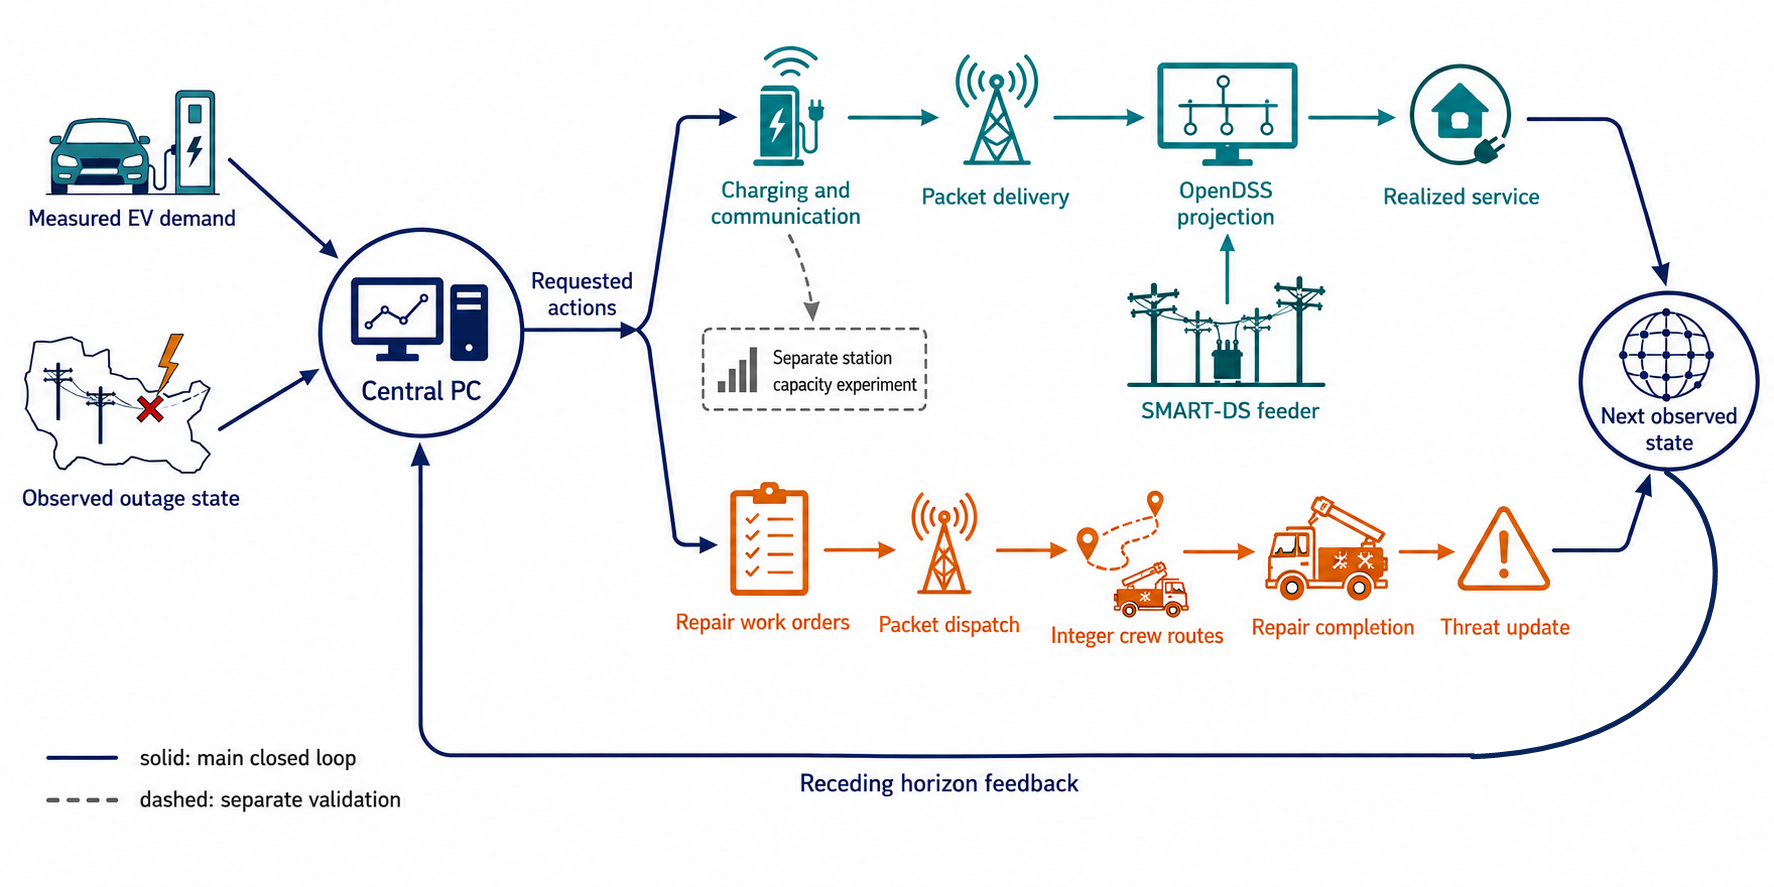
\includegraphics[width=\textwidth]{fig_executable_system.png}
\caption{\DIFaddFL{Executable PC closed loop.  Boulder charging demand and EAGLE-I outage
states inform central PC.  Requested service actions pass through packet
delivery and SMART-DS/OpenDSS projection.  Repair work orders pass through
packet dispatch, integer routing, and recorded completion events.  Realized
service and threat updates form the next observed state.  The dashed path
denotes the separate station capacity experiment and is not part of the primary
4,096-scenario loop.}}
\label{fig:executable-system}
\end{figure*}

\begin{table*}[t]
\centering
\caption{Independent evidence sources and their distinct roles}
\label{tab:evidence-sources}
\begin{tabular}{p{0.17\textwidth}p{0.18\textwidth}p{0.20\textwidth}p{0.35\textwidth}}
\toprule
Source & Scale & Observed fields & Role in this study \\
\midrule
City of Boulder EV sessions & 148,136 transactions from 50 stations between 2018 and 2023 & Arrival time, charging duration, energy (kWh), station and address & Measured charging demand with calendar periods for training, selection, and testing \\
EAGLE-I & 249,316,543 national rows with 819,528 retained in Boulder and six adjacent counties between 2014 and 2025 & County, UTC timestamp, customers out & Power state persistence, event and recovery distributions, and uncertainty bounds with missing rows preserved \\
SMART-DS SFO P1U feeder & 80 buses, 219 nodes, 27 loads, 67 lines, 13 transformers & OpenDSS circuit, equipment and peak load operating point & Online projection for all primary policy hours and the integrated electrical stress test \\
Packet and route models & 12,000 packet stress rows and 4,096 paired main scenarios with up to 36 jobs and four crews & Queue events, retries, deadlines, backup, integer crews, travel, service and completion times & Requested controls and threat updates after a recorded repair completion event \\
\bottomrule
\end{tabular}
\end{table*}


\DIFadd{The primary demand source is the City of Boulder Electric Vehicle Charging
Station Data under a CC0 license.  Its metadata defines one
row as one transaction and provides local transaction time, station identity,
charging duration, and delivered energy.  The local archive contains all
148,136 transactions released from 2018 through }\DIFaddend 2023\DIFdelbegin \DIFdel{collection contains 38}\DIFdelend \DIFaddbegin \DIFadd{, with 50 station records and
1}\DIFaddend ,\DIFdelbegin \DIFdel{310}\DIFdelend \DIFaddbegin \DIFadd{252}\DIFaddend ,\DIFdelbegin \DIFdel{226 raw trip
records.  Invalid location identifiers, trips outside the calendar year, and
implausible trip distances are removed.
This leaves 36, 879, 930 valid trips.
Trips are aggregated to hourly values over 263 zones, which gives 8760 time
steps.  For each hour and zone, the data construction computes pickup activity, drop off activity, trip mileage, charging energy demand, and origin destination
flows}\DIFdelend \DIFaddbegin \DIFadd{719.654 measured positive kWh.  Four records lack an end time, 16,113
report zero energy, no duplicate source identifier or full row was found, and
no negative energy was retained.  Arrival counts are exact transaction counts
by start hour.  Session energy is measured.  Its hourly load profile is obtained
by spreading each session's energy uniformly over the reported
charging duration.  Conservation checks recover all 148,136 arrivals and the
measured positive energy to within 0.001 kWh}\DIFaddend .

\DIFdelbegin \DIFdel{Let $d_{\tau i}^{\mathrm{mile}}$ denote the total trip distance assigned to zone $i$ in hour $\tau$.  Charging energy is estimated from this mileage by
}%DIFDELCMD < \begin{equation}
%DIFDELCMD < e_{\tau i}
%DIFDELCMD < =\pi_{\mathrm{EV}}\epsilon_{\mathrm{mile}}d_{\tau i}^{\mathrm{mile}},
%DIFDELCMD < \label{eq:energy-conversion}
%DIFDELCMD < \end{equation}
%DIFDELCMD < %%%
\DIFdel{where $\pi_{\mathrm{EV}}=0.18$ is the
assumed electric vehicle share and $\epsilon_{\mathrm{mile}}=0.24$ kWh per mile is the
energy use coefficient for
electric mobility.  The factor $\pi_{\mathrm{EV}}$ converts observed travel
mileage into electric mobility mileage, and $\epsilon_{\mathrm{mile}}$ converts
electric mobility mileage into charging energy.  The same conversion is applied
to all methods.  The origin destination matrix is converted to a top neighbor
graph and normalized.  Feeder capacityand communication capacity indicators are
deterministic functions of historical load intensity.
The resulting data set is large, public, and directly reproducible in the digital twin.  }%DIFDELCMD < 

%DIFDELCMD < \begin{table}[t]
%DIFDELCMD < \centering
%DIFDELCMD < %%%
%DIFDELCMD < \caption{%
{%DIFAUXCMD
\DIFdelFL{Data construction used by the digital twin}}
%DIFAUXCMD
%DIFDELCMD < \label{tab:data}
%DIFDELCMD < \begin{tabular}{lr}
%DIFDELCMD < \toprule
%DIFDELCMD < %%%
\DIFdelFL{Quantity }%DIFDELCMD < & %%%
\DIFdelFL{Value }%DIFDELCMD < \\
%DIFDELCMD < \midrule
%DIFDELCMD < %%%
\DIFdelFL{Raw trips }%DIFDELCMD < & %%%
\DIFdelFL{38, 310, 226 }%DIFDELCMD < \\
%DIFDELCMD < %%%
\DIFdelFL{Valid trips after filtering }%DIFDELCMD < & %%%
\DIFdelFL{36, 879, 930 }%DIFDELCMD < \\
%DIFDELCMD < %%%
\DIFdelFL{Zones }%DIFDELCMD < & %%%
\DIFdelFL{263 }%DIFDELCMD < \\
%DIFDELCMD < %%%
\DIFdelFL{Hourly states }%DIFDELCMD < & %%%
\DIFdelFL{8760 }%DIFDELCMD < \\
%DIFDELCMD < %%%
\DIFdelFL{Historical window }%DIFDELCMD < & %%%
\DIFdelFL{12 hours }%DIFDELCMD < \\
%DIFDELCMD < %%%
\DIFdelFL{Rollout horizon }%DIFDELCMD < & %%%
\DIFdelFL{6 hours }%DIFDELCMD < \\
%DIFDELCMD < %%%
\DIFdelFL{Electric vehicle share $\pi_{\mathrm{EV}}$ }%DIFDELCMD < & %%%
\DIFdelFL{0.18 }%DIFDELCMD < \\
%DIFDELCMD < %%%
\DIFdelFL{Energy use coefficient $\epsilon_{\mathrm{mile}}$ }%DIFDELCMD < & %%%
\DIFdelFL{0.24 kWh per mile }%DIFDELCMD < \\
%DIFDELCMD < \bottomrule
%DIFDELCMD < \end{tabular}
%DIFDELCMD < \end{table}
%DIFDELCMD < 

%DIFDELCMD < %%%
\DIFdel{Table~\ref{tab:data} summarizes the quantities that enter the digital twin.  The
raw trip records are reduced to an hourly state tensor, but the tensor still
preserves demand variation from a full year of city scale mobility records.  The
charging and communication quantities remain fixed deterministic transformations
of the
same processed activity data, which keeps the policy comparison tied to one common operating environment.
}%DIFDELCMD < 

%DIFDELCMD < %%%
\subsection{\DIFdel{Compared policies}}
%DIFAUXCMD
\addtocounter{subsection}{-1}%DIFAUXCMD
%DIFDELCMD < 

%DIFDELCMD < %%%
\DIFdel{The forecasting history is twelve hours and the rollout horizon is six hours.  The chronological data split uses the first part }\DIFdelend \DIFaddbegin \DIFadd{Time was split before model fitting.  The period from 2018 through 2021 was used
}\DIFaddend for training, \DIFdelbegin \DIFdel{the middle part
for validation, and the final part for testing.  The graph recurrent predictor
is trained on a graphics processor.
The tested operating policies are static
allocation,greedy current state allocation,neural rollout,PC rollout, and an
oracle reference.  Static allocation uses historical averages.  Greedy
allocation reacts only to the current grid and charging state.
Neural rollout
uses the same forecast as PC rollout and assigns restoration from the current
threat field.  The oracle uses future realized demand and threat values and is
included only as a reference.  }\DIFdelend \DIFaddbegin \DIFadd{2022 was used for model selection, and 2023 was used for final
testing.  No random row split crosses this
calendar boundary.  A second five fold spatial test withheld contiguous
west to east station blocks from target fitting.  In that inductive deployment
test, a held out station's calibration before 2022 and observed 1, 24, and 168 h
lags were permitted, but its target values never entered coefficient fitting.
}\DIFaddend 

\DIFdelbegin \DIFdel{Threat scenarios are generated in four groups.  The nominal group contains
small perturbations.  The single domain group perturbs one of mobility, power,
or communication.
The cascading group allows cross domain propagation.  The unseen compound group uses stronger and longer disruptions than those used in the
nominal and single domain cases.
Each group contains the same number of
scenarios.  Every policy is evaluated on the same realized demand and threat
sequence.  }\DIFdelend \DIFaddbegin \DIFadd{Power event evidence came from the CC BY 4.0 EAGLE-I release
}\cite{brelsford2024eaglei}\DIFadd{.  The source record contained 17 files and
249,316,543 rows.  Preprocessing retained
819,528 observations for Boulder County and its six adjacent counties,
including 171,187 Boulder observations.  EAGLE-I timestamps are UTC and were
converted to America/Denver only for alignment with local charging records.
Because the source omits zero outage records and cannot distinguish a true zero
from a collection gap, absent county and time pairs were preserved as missing
rather than silently imputed as zero.  Events were evaluated at 50, 100, and
500 customers out.  At the 50-customer threshold, 2,535 events had median
duration 1.75 h and 90th percentile duration 6.5 h.  The post peak half recovery
time was observable for 19.6\% of events and had median 0.75 h.  These traces
inform a scenario distribution, not station level failure labels or utility
work orders.
}\DIFaddend 

The \DIFdelbegin \DIFdel{threat generator selects initial affected zones with probabilities
proportional to historical demand.  This makes disruptions more likely to enter
busy charging service zones while still allowing all zones to appear across the scenario set.
For scenario class $g$, the latent threat intensity follows
}%DIFDELCMD < \begin{equation}
%DIFDELCMD < b_{h+1}=
%DIFDELCMD < \Pi_{[0,1]^N}\left(\kappa_0 b_h+\rho_g A b_h+\nu_h\right),
%DIFDELCMD < \label{eq:scenario}
%DIFDELCMD < \end{equation}
%DIFDELCMD < %%%
\DIFdel{where $\kappa_0$ is temporal persistence, $\rho_g$ controls spatial spread, and $\nu_h$ is a bounded multiplicative perturbation.Mobility, power, and communication threat fields are obtained by domain specific scaling of $b_h$.  In cascading and unseen compound scenarios, cross domain terms are added before
projection, }%DIFDELCMD < \begin{align}
%DIFDELCMD < z_{h}^{c} &\leftarrow
%DIFDELCMD < \Pi_{[0,1]^N}\left(z_h^c+\tau_{pc}z_h^p+\tau_{rc}Az_h^r\right),\\
%DIFDELCMD < z_{h}^{r} &\leftarrow
%DIFDELCMD < \Pi_{[0,1]^N}\left(z_h^r+\tau_{cr}z_h^c\right),\\
%DIFDELCMD < z_{h}^{p} &\leftarrow
%DIFDELCMD < \Pi_{[0,1]^N}\left(z_h^p+\tau_{cp}Az_h^c\right).
%DIFDELCMD < \end{align}
%DIFDELCMD < %%%
\DIFdel{The coefficients $\tau_{pc}$,
$\tau_{rc}$, $\tau_{cr}$,
and $\tau_{cp}$ specify
power to communication, mobility to communication, communication to
mobility,
and communication to power propagation strength.
}\DIFdelend \DIFaddbegin \DIFadd{independent electrical test uses one complete SMART-DS v1.0 San Francisco
P1U feeder and its unmodified OpenDSS model.  The solved circuit contains 80
buses, 219 nodes, 27 loads,
67 lines, and 13 transformers.  Eighteen nodes already deenergized in the
released base case are identified and excluded from active voltage minima.
They are not counted as failures caused by EV action.  The base active node voltage
minimum is 0.989 p.u. and maximum line loading is 0.913 p.u.  Requested EV
actions are aggregated as balanced three phase, wye connected constant $PQ$
increments at the 17 eligible three phase loads.  Active power is the executed
station request and reactive power follows a 0.98 lagging power factor.  }\DIFaddend The
\DIFdelbegin \DIFdel{scenario generator follows
the propagation model in \eqref{eq:propagation}, while the controller receives
the realized state and applies its own rollout rule.  The shared scenario stream
ensures that differences in Table~\ref{tab:rollout} come from policy decisions
rather than from different disturbance draws.
}\DIFdelend \DIFaddbegin \DIFadd{released load voltage level (0.48 or 12.47 kV) and base load parameters are
otherwise unchanged.  Twenty
station to load mappings are prepared in advance.  Mapping $s\bmod20$ is
shared by all six policies in scenario $s$ and recorded in the scenario table.
At every simulated hour, station level executable charging is aggregated at the
assigned loads, OpenDSS solves the unprojected action, and a bisection backtracks
its common fraction until voltage lies in $[0.95,1.05]$ p.u., line loading is at
most 1.0 p.u., and the circuit converges.  Only this projected energy enters
served energy and backlog equations.  This gate validates the electrical
feasibility of a proposed charging action.  It does not simulate feeder
topology reconfiguration, switching or breaker operations, fault isolation,
feeder resupply, or equipment parameter changes after repair.  The experiment
therefore studies charging service restoration under a fixed feeder topology.
}\DIFaddend 

\DIFdelbegin \DIFdel{For each scenario, all five policies are evaluated on the same demand horizon
and threat horizon.  The reported cost is the sum of mobility delay,unserved
charging demand,communication loss,feeder margin violation, and cascade
interaction terms appearing in \eqref{eq:stage}.  Service continuity is computed
as served mobility divided by total mobility over the horizon.  The final tables
report mean values across all evaluated scenarios, and the scenario class table
keeps the same aggregation within each threat group.  }\DIFdelend \DIFaddbegin \subsection{\DIFadd{Demand forecasting and spatial transfer}}
\DIFaddend 

\DIFdelbegin %DIFDELCMD < \begin{table}[t]
%DIFDELCMD < \centering
%DIFDELCMD < %%%
%DIFDELCMD < \caption{%
{%DIFAUXCMD
\DIFdelFL{Policies compared in the rollout evaluation}}
%DIFAUXCMD
%DIFDELCMD < \label{tab:policies}
%DIFDELCMD < \begin{tabular}{p{0.28\linewidth}p{0.62\linewidth}}
%DIFDELCMD < \toprule
%DIFDELCMD < %%%
\DIFdelFL{Policy }%DIFDELCMD < & %%%
\DIFdelFL{Decision information }%DIFDELCMD < \\
%DIFDELCMD < \midrule
%DIFDELCMD < %%%
\DIFdelFL{Static }%DIFDELCMD < & %%%
\DIFdelFL{Historical average service and restoration allocation }%DIFDELCMD < \\
%DIFDELCMD < %%%
\DIFdelFL{Greedy }%DIFDELCMD < & %%%
\DIFdelFL{Current feeder, charging demand , and current threat field }%DIFDELCMD < \\
%DIFDELCMD < %%%
\DIFdelFL{Neural rollout }%DIFDELCMD < & %%%
\DIFdelFL{Graph forecast with current threat restoration }%DIFDELCMD < \\
%DIFDELCMD < %%%
\DIFdelFL{PC rollout }%DIFDELCMD < & %%%
\DIFdelFL{Graph forecast with future cascade envelope restoration }%DIFDELCMD < \\
%DIFDELCMD < %%%
\DIFdelFL{Oracle }%DIFDELCMD < & %%%
\DIFdelFL{Realized future demand and threat values for reference }%DIFDELCMD < \\
%DIFDELCMD < \bottomrule
%DIFDELCMD < \end{tabular}
%DIFDELCMD < \end{table}
%DIFDELCMD < %%%
\DIFdelend \DIFaddbegin \begin{table}[t]
\centering
\caption{Calendar split test performance on measured Boulder charging sessions in 2023}
\label{tab:real-ev-forecast}
\begin{tabular}{lrrrr}
\toprule
Method & \multicolumn{2}{c}{Arrivals} & \multicolumn{2}{c}{Energy (kWh)} \\
 & MAE & RMSE & MAE & RMSE \\
\midrule
Historical mean & 0.137 & 0.517 & 1.101 & 3.026 \\
Weekly seasonal & 0.156 & 0.637 & 1.130 & 3.299 \\
Persistence & 0.175 & 0.678 & 1.059 & 3.186 \\
Graph recurrent forecaster & 0.110 & 0.527 & 0.945 & 3.113 \\
\bottomrule
\end{tabular}
\end{table}

\DIFaddend 

\DIFaddbegin \DIFadd{Table~\ref{tab:real-ev-forecast} reports the fixed 2023 temporal test.  The
graph recurrent forecaster achieved arrival MAE 0.110 and energy MAE 0.945 kWh,
compared with 0.137 and 1.101 kWh for the historical mean.  Its energy RMSE
(3.113 kWh) did not beat the historical mean (3.026 kWh), so no uniform metric
dominance is claimed.  Across three training runs, arrival MAE ranged from 0.1096 to
0.1099 and energy MAE from 0.9452 to 0.9468 kWh.
}

\DIFadd{The spatial test pooled all five held out
blocks and six horizons, the spatial ridge model reduced energy MAE from 1.130
to 1.054 kWh and RMSE from 2.928 to 2.272 kWh relative to station specific weekly
history.  Arrival RMSE also decreased from 0.557 to 0.440, but arrival MAE
(0.161) was worse than the pooled calendar mean (0.139).  Thus the measured data
forecast supports temporal deployment and improves several unseen station
endpoints.  Arrival MAE remains higher at sparse stations, which identifies the
forecast condition for interpreting the decision study.
}

\subsection{\DIFadd{Propagation calibration and policy comparison}}

\begin{table}[t]
\centering
\caption{Propagation coefficients and prespecified uncertainty set}
\label{tab:calibrated-uncertainty}
\begin{tabular}{lrrl}
\toprule
Parameter & Central & Interval & Evidence class \\
\midrule
$\rho_r$ & 0.728 & [0.546, 0.911] & estimated \\
$\sigma$ & 0.233 & [0.116, 0.349] & estimated \\
$\rho_p$ & 0.772 & [0.754, 0.787] & estimated \\
$\tau_{pr}$ & 0.000 & [0.000, 0.032] & estimated observational \\
$\tau_{pc}$ & 0.427 & [0.169, 0.551] & constructed \\
$\rho_c$ & 0.500 & [0.300, 0.800] & sensitivity only \\
$\tau_{rc}$ & 0.040 & [0.000, 0.080] & sensitivity only \\
$\tau_{cr}$ & 0.080 & [0.000, 0.160] & sensitivity only \\
$\tau_{cp}$ & 0.040 & [0.000, 0.080] & sensitivity only \\
\bottomrule
\end{tabular}
\end{table}


\DIFadd{The coefficient ledger in }\DIFaddend Table~\DIFdelbegin \DIFdel{\ref{tab:policies} clarifies the main comparison .  Neural rollout and PC
rollout have the
same forecast input.  Their difference is the restoration
allocation.  This design keeps the experiment aligned with the analysis in
Theorem 1 and Corollary }\DIFdelend \DIFaddbegin \DIFadd{\ref{tab:calibrated-uncertainty} distinguishes
estimated, observational, constructed, and sensitivity range quantities.  A
nonnegative station deficit regression estimated road and mobility persistence and
spatial spread from }\DIFaddend 1,\DIFdelbegin \DIFdel{where the performance gap is connected to future
threat growth rather than to a different demand estimator.  }\DIFdelend \DIFaddbegin \DIFadd{268,661 training samples.  On 3,108 aligned 2023 test
hours, its road state RMSE was 0.306 versus 0.374 for persistence.  EAGLE-I
estimated power persistence at 0.772 with a day block bootstrap interval
$[0.754,0.787]$.  The aligned coefficient from power state to EV deficit was effectively
zero with upper interval 0.032, providing no evidence for a strong direct
conditional association.  The packet model constructed the
power to communication interval.  Directions without joint field traces span
sign constrained sensitivity ranges including zero.
}\DIFaddend 

\DIFdelbegin \subsection{\DIFdel{Computation}}
%DIFAUXCMD
\addtocounter{subsection}{-1}%DIFAUXCMD
%DIFDELCMD < 

%DIFDELCMD < %%%
\DIFdel{The experiments require two types of computation.
The graph forecasting model
uses parallel tensor operations on a graphics processor.  The scenario
evaluation uses many independent rollout simulations and is therefore executed
with parallel central processor cores.  This division keeps the graphics
processor busy only during model training and moves scenario evaluation to central processor cores.  The final evaluation includes thousands of base
scenariosand an additional set of power oriented stress cases.  Reduced
examples can be run on ordinary hardware, but the complete repeated experiment
is substantially more convenient on a shared computing platform with both
graphics and central processor resources.
}\DIFdelend \DIFaddbegin \DIFadd{The primary central PC policy evaluates multistep propagation under the
calibrated central matrix.  The robust extension evaluates 21 central/endpoint
matrices and allocates using the smallest predicted marginal action benefit.
In the realized dynamics,
each coefficient was sampled independently from its prespecified interval for
each scenario.  Forecast matched, central PC, and robust PC received the same
selected demand forecast, current threat observation, backlog, and realized
past.  Static instead used historical station means, greedy used the common
forecast but formed a direct current threat route, and the oracle alone
received future innovations.  The forecast matched baseline uses no
propagation matrix.  It scores the common
finite route portfolio from current threat and forecast exposure only.  Central
PC propagates the calibrated central matrix, whereas robust PC minimizes the
worst score over the 21 matrix set.  Thus forecast matched is not central PC.
Table~\ref{tab:policy-definitions} fixes the information and execution contract
for all six policies.  The oracle alone receives future innovations.  The
primary family comprised central PC versus the matched baseline for total cost
overall and in four prespecified threat classes.  We used 4,096 paired scenarios
(1,024 per class), paired bootstrap intervals with 20,000 resamples, paired
$t$ tests, two sided Wilcoxon tests, and Holm
correction across the five classwise tests.
Supplementary Table S1 reports each value, unit, role, calibration rule,
selection source, and tested range.
}\DIFaddend 

\DIFdelbegin %DIFDELCMD < \begin{table}[t]
%DIFDELCMD < \centering
%DIFDELCMD < %%%
%DIFDELCMD < \caption{%
{%DIFAUXCMD
\DIFdelFL{Training and rollout computation settings}}
%DIFAUXCMD
%DIFDELCMD < \label{tab:compute}
%DIFDELCMD < \begin{tabular}{lr}
%DIFDELCMD < \toprule
%DIFDELCMD < %%%
\DIFdelFL{Quantity }%DIFDELCMD < & %%%
\DIFdelFL{Value }%DIFDELCMD < \\
%DIFDELCMD < \midrule
%DIFDELCMD < %%%
\DIFdelFL{Trainable parameters }%DIFDELCMD < & %%%
\DIFdelFL{30}\DIFdelendFL \DIFaddbeginFL \begin{table*}[t]
\centering
\caption{Policy information and execution contract.  ``Current'' means the
observation available at the decision hour.  The common route portfolio contains
routes induced by static, greedy, forecast-matched, central-PC, robust-PC, and
uniform priorities.  Future innovations are never revealed to deployable
policies.}
\label{tab:policy-definitions}
\scriptsize
\setlength{\tabcolsep}{2.4pt}
\begin{tabular}{p{0.10\textwidth}p{0.10\textwidth}p{0.10\textwidth}p{0.09\textwidth}p{0.125\textwidth}p{0.085\textwidth}p{0.155\textwidth}p{0.125\textwidth}}
\toprule
Policy & Demand information & Threat/backlog & Multi-step transition rollout & Transition matrix used & Future innovations & Repair-route rule & Common execution gates \\
\midrule
Static & Historical station mean & Backlog only for charging & No & None & No & Direct route from static priority & Yes \\
Greedy & Common forecast & Current threat and backlog & No & None & No & Direct route from current-threat priority & Yes \\
Forecast-matched & Common forecast & Current threat and backlog & No & None & No & Current-exposure score over common portfolio & Yes \\
Central PC & Common forecast & Current threat and backlog & Yes & Calibrated central $M$ & No & Central-transition score over common portfolio & Yes \\
Robust PC (extension) & Common forecast & Current threat and backlog & Yes & Worst score over 21 declared matrices & No & Worst-transition score over common portfolio & Yes \\
Oracle & Realized future demand & Current threat and backlog & Yes & Central $M$ & Yes & Direct route from oracle priority & Yes \\
\bottomrule
\end{tabular}
\end{table*}


\begin{table}[t]
\centering
\caption{Central PC compared with the same service score without threat propagation, followed by all policy means. Positive reduction denotes lower cost than forecast matched. $\Delta$ is central minus matched cost. Intervals are paired marginal intervals. All policies share 4,096 scenarios and the oracle alone observes future demand and innovations.}
\label{tab:robust-boulder}
\footnotesize
\setlength{\tabcolsep}{3pt}
\resizebox{\columnwidth}{!}{%
\begin{tabular}{@{}lrrrr@{}}
\toprule
Group & Pairs & Reduction (\%) & $\Delta$ & $\Delta$ 95\% CI \\
\midrule
All & 4096 & 0.1027 & -1.1436 & [-1.5257, -0.7704] \\
Nominal & 1024 & -0.0002 & 0.0013 & [-0.0042, 0.0075] \\
Single domain & 1024 & 0.0132 & -0.1021 & [-0.2602, 0.0510] \\
Cascade & 1024 & 0.0741 & -0.7946 & [-1.7624, 0.1327] \\
OOD compound & 1024 & 0.1979 & -3.6789 & [-4.8554, -2.5890] \\
\bottomrule
\end{tabular}
}
\vspace{3pt}
\begin{tabular}{@{}lrr@{}}
\toprule
Policy & Mean cost & Reduction (\%) \\
\midrule
Forecast matched & 1113.68 & 0.0000 \\
Central PC & 1112.54 & 0.1027 \\
Robust PC & 1112.90 & 0.0697 \\
Exposure matched & 1120.23 & -0.5885 \\
Exposure central & 1124.63 & -0.9832 \\
Static & 1202.74 & -7.9970 \\
Greedy & 1122.54 & -0.7960 \\
Oracle & 1053.67 & 5.3887 \\
\bottomrule
\end{tabular}
\end{table}


\DIFaddFL{Table~\ref{tab:robust-boulder} reports the primary paired comparison and the
policy summary.  Central PC reduced mean total cost by 0.6327\% overall relative to the matched
baseline (paired difference $-6.2730$}\DIFaddendFL , \DIFdelbeginFL \DIFdelFL{220 }%DIFDELCMD < \\
%DIFDELCMD < %%%
\DIFdelFL{Training epochs }%DIFDELCMD < & %%%
\DIFdelFL{80 }%DIFDELCMD < \\
%DIFDELCMD < %%%
\DIFdelFL{Training repetitions }%DIFDELCMD < & %%%
\DIFdelFL{3 }%DIFDELCMD < \\
%DIFDELCMD < %%%
\DIFdelFL{Scenario classes }%DIFDELCMD < & %%%
\DIFdelFL{4 }%DIFDELCMD < \\
%DIFDELCMD < %%%
\DIFdelFL{Scenarios per class }%DIFDELCMD < & %%%
\DIFdelFL{1024 }%DIFDELCMD < \\
%DIFDELCMD < %%%
\DIFdelFL{Policies per scenario }%DIFDELCMD < & %%%
\DIFdelFL{5 }%DIFDELCMD < \\
%DIFDELCMD < %%%
\DIFdelFL{Power stress and sensitivity cases }%DIFDELCMD < & %%%
\DIFdelFL{9 }%DIFDELCMD < \\
%DIFDELCMD < %%%
\DIFdelFL{Central processor cores for evaluation }%DIFDELCMD < & %%%
\DIFdelFL{32 }%DIFDELCMD < \\
%DIFDELCMD < %%%
\DIFdelFL{Base evaluation simulation time }%DIFDELCMD < & %%%
\DIFdelFL{1.10 seconds }%DIFDELCMD < \\
%DIFDELCMD < \bottomrule
%DIFDELCMD < \end{tabular}
%DIFDELCMD < \end{table}
%DIFDELCMD < %%%
\DIFdelend \DIFaddbegin \DIFadd{95\% bootstrap CI
$[-7.0372,-5.5195]$).  The Holm adjusted paired $t$ and Wilcoxon probabilities
were $3.84\times10^{-56}$ and $9.76\times10^{-101}$, respectively.  All four
prespecified groups had negative intervals, with reductions of 0.0020\% in
nominal, 0.0433\% in single domain, 0.6502\% in cascade, and 1.1296\% in OOD
compound cases.  The nominal effect is statistically distinguishable in these
simulated pairs but operationally negligible.  The intervals quantify Monte
Carlo scenario uncertainty, not variation across real utility systems.
}\DIFaddend 

The \DIFdelbegin \DIFdel{computation settings in Table~\ref{tab:compute} explain why the evaluation
was run as a repeated parallel experiment rather than as a small example.  The forecasting model is modest in size, while the evaluation requires repeated
closed loop rollouts over many disruptions.  The runtime is controlled by the independence of scenario rollouts and by distributing them over central
processor cores.
}\DIFdelend \DIFaddbegin \DIFadd{robust extension had higher mean cost than central PC (986.85 versus
985.17).  The robust minus central difference was 1.6830 with 95\% CI
$[1.3298,2.0508]$, or a 0.1708\% penalty.  Its 95th percentile cost was equal
to central PC (2381.08), its 99th percentile was 7.47 lower, but its CVaR at
95\% and 99\% was 4.48 and 3.19 higher, respectively, and the maximum was equal
(4084.41).  Robust PC won 3.83\%, tied 88.50\%, and lost 7.67\% of paired
scenarios.  These diagnostics do not support either an average cost or a
coherent tail risk advantage for worst set scoring, so robust PC is retained
only as a sensitivity extension.  Central PC reduced cost by 7.885\% relative
to static allocation.  The oracle alone received future innovations.  Its mean
cost was 896.01, leaving central PC with a 9.95\%
policy to oracle gap.  The oracle is therefore an information value
reference rather than evidence of near optimality.
}\DIFaddend 

\DIFdelbegin \subsection{\DIFdel{Empirical results}}
%DIFAUXCMD
\addtocounter{subsection}{-1}%DIFAUXCMD
\DIFdelend \DIFaddbegin \begin{table}[t]
\centering
\caption{Objective sensitivity of central PC relative to forecast matched. All rows use the same 1,024 scenario inputs. Candidate routes are selected again under each stated objective. Reference is the corresponding subset of the primary experiment, not its full 4,096 pairs.}
\label{tab:objective-sensitivity}
\footnotesize
\setlength{\tabcolsep}{3pt}
\resizebox{\columnwidth}{!}{%
\begin{tabular}{@{}lrr@{}}
\toprule
Weights & Reduction (\%) & Difference (95\% CI) \\
\midrule
Reference & 0.0995 & -1.1299 [-1.9426, -0.3834] \\
$2\times$ mobility & 0.1028 & -1.1782 [-2.0284, -0.3950] \\
$2\times$ unserved energy & 0.0597 & -1.1458 [-2.0653, -0.3006] \\
$2\times$ communication & 0.1029 & -1.3283 [-2.3910, -0.3448] \\
$2\times$ power service & 0.1264 & -1.4710 [-2.5631, -0.4754] \\
$0.5\times$ cascade & 0.0810 & -0.8553 [-1.5909, -0.1857] \\
\bottomrule
\end{tabular}
}
\end{table}

\DIFaddend 

\DIFdelbegin %DIFDELCMD < \begin{figure}[t]
%DIFDELCMD < %%%
\DIFdelendFL \DIFaddbeginFL \DIFaddFL{Table~\ref{tab:objective-sensitivity} shows that changing one objective
weight at a time did not reverse the central PC
comparison with forecast matched.  The reduction ranged from 0.4105\% to
0.7978\%, and every paired bootstrap interval remained below zero.  These tests
on fixed trajectories assess evaluation weight dependence.  They do not claim that a
policy optimized again for each alternative objective would select the same route.
}

\begin{figure*}[t]
\DIFaddendFL \centering
\DIFdelbeginFL %DIFDELCMD < 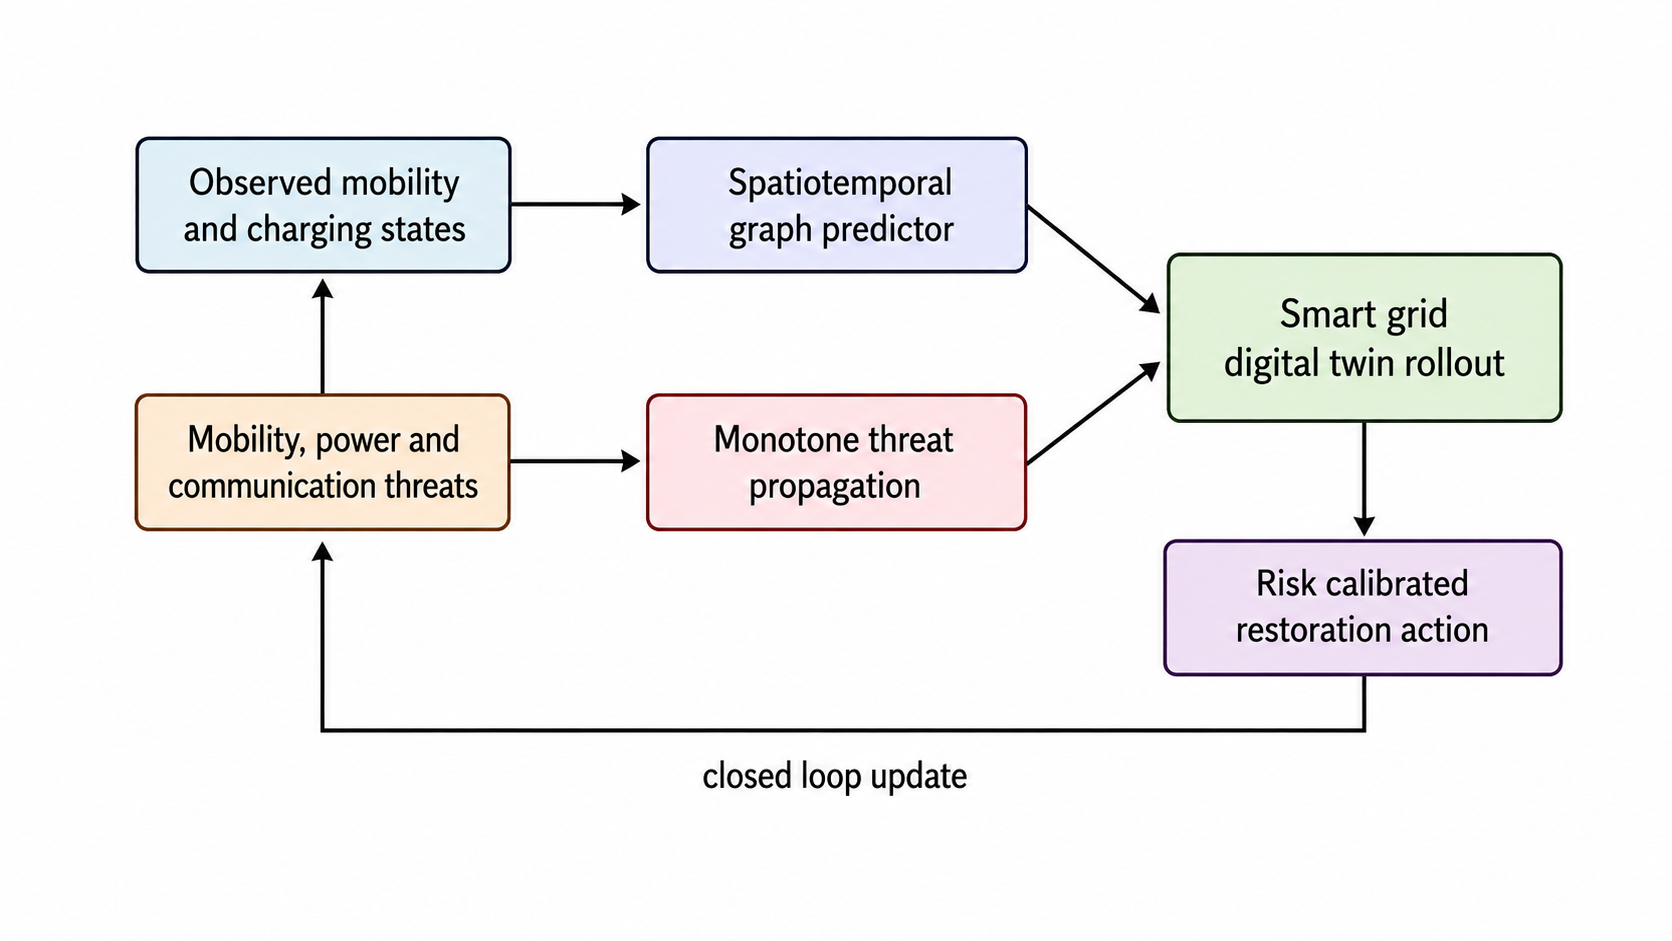
\includegraphics[width=\linewidth,trim=90 85 90 90,clip]{f1.png}
%DIFDELCMD < %%%
\DIFdelendFL \DIFaddbeginFL 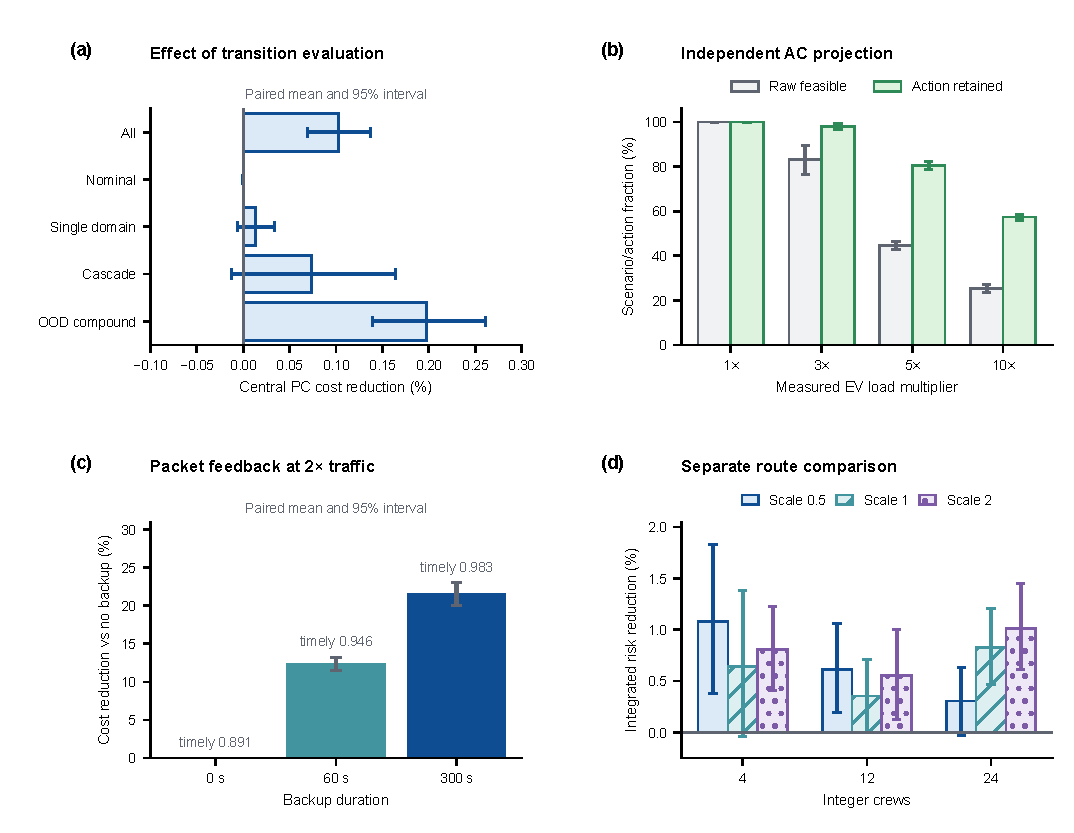
\includegraphics[width=\textwidth]{fig_operational_evidence.pdf}
\DIFaddendFL \caption{\DIFaddbeginFL\DIFaddFL{Decision and execution evidence.  Panel (a) reports the central PC cost
reduction relative to the forecast matched baseline.  Filled intervals show
paired means and bootstrap confidence limits for each threat class and for all
scenarios.  Panel (b) reports raw distribution system feasibility and the
fraction of requested EV action retained after projection.  Panel (c) reports
the cost reduction from backup power under increased packet traffic, with the
mean fraction of actions delivered on time printed above each bar.  Panel (d)
reports integrated risk reduction when executable routes are evaluated before
selection.  Exact sample sizes, confidence intervals, and adjusted tests are
reported in the surrounding tables.}\DIFaddendFL}
\label{fig:operational-evidence}
\end{figure*}
\DIFaddend 

\DIFdelbegin %DIFDELCMD < \input{table_rollout}
%DIFDELCMD < %%%
\DIFdelend \DIFaddbegin \DIFadd{Figure~\ref{fig:operational-evidence} places the primary transition comparison
beside the electrical, communication, and crew execution results.  The panels
use the same values and sample definitions as the corresponding tables.
}\DIFaddend 

\DIFdelbegin %DIFDELCMD < \begin{figure}[t]
%DIFDELCMD < \centering
%DIFDELCMD < 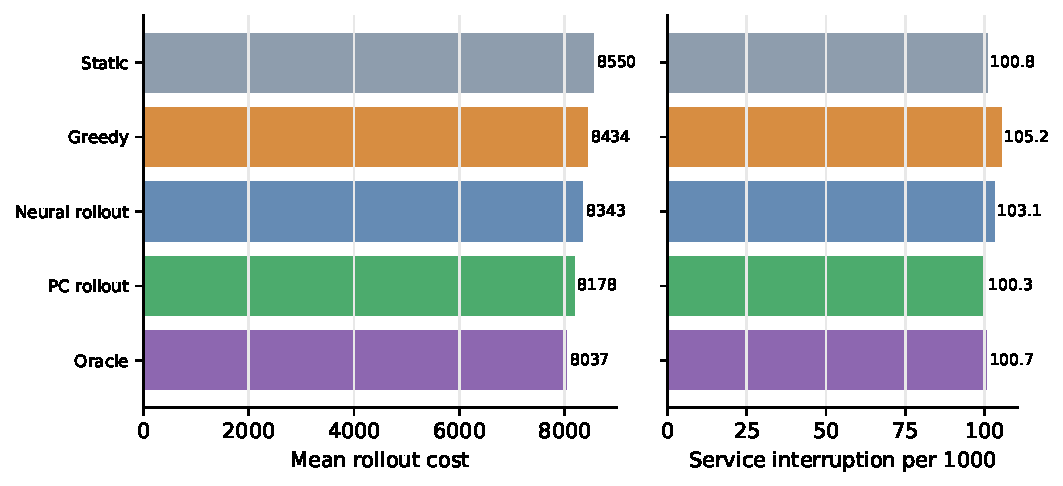
\includegraphics[width=0.98\linewidth]{fig_policy_bubbles.pdf}
%DIFDELCMD < %%%
%DIFDELCMD < \caption{%
{%DIFAUXCMD
\DIFdelFL{Mean cost and service interruption for the compared policies.}}
%DIFAUXCMD
%DIFDELCMD < \label{fig:bubbles}
%DIFDELCMD < \end{figure}
%DIFDELCMD < %%%
\DIFdelend \DIFaddbegin \subsection{\DIFadd{Electrical and mobility execution}}
\DIFaddend 

\DIFdelbegin %DIFDELCMD < \input{table_threat_class}
%DIFDELCMD < %%%
\DIFdelend \DIFaddbegin \begin{table}[t]
\centering
\caption{Electrical projection and repair completion in the integrated experiments. Primary includes eight policies and stress includes six. Action retention is the mean hourly fraction. Job completion is the mean scenario fraction of requested jobs completed within the horizon.}
\label{tab:integrated-execution}
\footnotesize
\setlength{\tabcolsep}{3pt}
\resizebox{\columnwidth}{!}{%
\begin{tabular}{@{}lrrrr@{}}
\toprule
Condition & Pairs & AC hours & Raw infeas. & After proj. \\
\midrule
Measured load & 4,096 & 196,608 & 0 & 0 \\
$20\times$ EV load & 1,024 & 36,864 & 348 & 0 \\
\bottomrule
\end{tabular}
}
\vspace{3pt}
\begin{tabular}{@{}lrr@{}}
\toprule
Condition & Action retained (\%) & Jobs completed (\%) \\
\midrule
Measured load & 100.00 & 81.05 \\
$20\times$ EV load & 99.80 & 81.12 \\
\bottomrule
\end{tabular}
\end{table}

\DIFaddend 

\DIFdelbegin \DIFdel{With the forecast fixed, }\DIFdelend \DIFaddbegin \DIFadd{Table~\ref{tab:integrated-execution} summarizes the feeder and crew outcomes in
the main loop.  The primary run with 4,096 scenarios made 147,456 online OpenDSS calls, one for each
scenario, policy, and hour.  At measured load, all raw actions were already feasible,
so projection retained 100\% of requested charging.  This feasibility
result but cannot by itself demonstrate feedback.  The companion $20\times$
stress run therefore used 1,024 paired scenarios and the same loop.  It produced
1,089 infeasible policy hours.  Projection reduced this count to zero,
retained 99.26\% of requested service on average, and placed 69,664.8 kWh of
curtailed energy into unserved demand/backlog rather than crediting it as served.
Thus the online adapter changes downstream state whenever the AC limit binds.
}

\begin{table}[t]
\centering
\caption{SMART-DS AC action projection (20 mappings, 24 hours each)}
\label{tab:smartds-action-loop}
\resizebox{\columnwidth}{!}{%
\begin{tabular}{lrrrr}
\toprule
EV load & Raw feasible (\%) & Action retained (\%) & Raw $V_{\min}$ & Raw line p.u. \\
\midrule
1$\times$ & 100.0 & 100.0 & 0.986 & 0.929 \\
3$\times$ & 83.1 & 98.0 & 0.977 & 0.968 \\
5$\times$ & 44.6 & 80.5 & 0.966 & 1.044 \\
10$\times$ & 25.4 & 57.3 & 0.938 & 1.361 \\
\bottomrule
\end{tabular}
}
\end{table}


\DIFadd{Table~\ref{tab:smartds-action-loop} extends the electrical comparison across
load multipliers.  The SMART-DS experiment comprised 20 randomized station to load mappings, 24
test hours, and four EV load multipliers (1,920 cases).  Raw actions were all
feasible at measured load.  At $3\times$, $5\times$, and $10\times$ load, raw
feasibility fell to 83.1\%, 44.6\%, and 25.4\%, whereas the action projection
retained 98.2\%, 81.1\%, and 57.7\% of requested EV power.  Every projected
case converged and met the voltage and line limits.  A separate test for all of 2023
used all 7,451 nonzero hours at $1\times$ and $3\times$ load (14,902 cases).
At $3\times$, 99.17\% of raw actions were feasible and projection retained
99.94\% on average.  All projected cases remained feasible.  The reported
curtailment is therefore produced inside the action path and not inferred from
a later voltage label.
}

\begin{table}[t]
\centering
\caption{Station choice under measured demand for 24 peak hours}
\label{tab:station-choice}
\resizebox{\columnwidth}{!}{%
\begin{tabular}{rrrrrr}
\toprule
Closure (\%) & No choice & Nearest & Logit & Coordinated & Extra km \\
\midrule
10 & 67.4 & 100.0 & 100.0 & 100.0 & 0.32 \\
20 & 55.8 & 100.0 & 100.0 & 100.0 & 0.50 \\
30 & 43.7 & 100.0 & 100.0 & 100.0 & 0.97 \\
\bottomrule
\end{tabular}
}
\end{table}


\DIFadd{Table~\ref{tab:station-choice} reports the station reassignment results.  Station
closure does not automatically imply abandoned charging.  A separate
capacity constrained flow model distinguished local service, rerouting, and
unserved demand across 24 observed peak hours.  Under measured demand and 10,
20, and 30\% closures, preserving the original station served only 67.4, 55.8,
and 43.7\% of energy.  Nearest, logit, and coordinated reassignment all served
100\% in these cases.  The coordinated solution required only 0.32, 0.50, and
0.97 km energy weighted extra distance.  Under $4\times$ demand, total
constructed capacity, rather than the choice model, became the limiting factor.
This stress result prevents the rerouting mechanism from creating fictitious
capacity.
}

\subsection{\DIFadd{Communication and crew execution}}

\DIFadd{The packet emulator is a finite buffer queue with first come, first served
discipline, discrete events, erasures, two retransmissions, backoff, a 500 ms control deadline,
and explicit backup duration.  An M/M/1 unit test at 10 packet/s arrival and
20 packet/s service reproduced the theoretical 100 ms mean latency with 0.269\%
relative error.  Across 12,000 station stress cases, the original algebraic
support proxy had Spearman correlation 0.860 but mean absolute error 0.243
against the simulated fraction of actions delivered on time, which confirms that the proxy
cannot replace packet dynamics.
}

\begin{table}[t]
\centering
\caption{Backup duration for central PC at $2\times$ packet traffic on 1,024 paired scenarios. Completion is the fraction of requested jobs completed. Cost differences compare the same policy with no backup.}
\label{tab:packet-feedback}
\footnotesize
\setlength{\tabcolsep}{3pt}
\resizebox{\columnwidth}{!}{%
\begin{tabular}{@{}lrrrr@{}}
\toprule
Backup & Timely action & Completion & Reduction (\%) & Difference 95\% CI \\
\midrule
0 s & 0.891 & 0.754 & 0.00 & Reference \\
60 s & 0.946 & 0.790 & 12.35 & [-186.05, -161.06] \\
300 s & 0.983 & 0.819 & 21.55 & [-323.85, -281.66] \\
\bottomrule
\end{tabular}
}
\end{table}


\DIFadd{Table~\ref{tab:packet-feedback} reports the effect of backup duration.
Equation~\eqref{eq:packet-derate} closes this evidence loop.  Under prespecified
$2\times$ traffic and 1,024 paired uncertain transition scenarios, 60 s backup
raised the mean timely action fraction to 0.938 and reduced central PC cost
by 10.54\% relative to no backup (difference CI $[-147.3,-126.8]$).  A 300 s
backup raised the fraction to 0.969 and reduced cost by 18.83\% (difference CI
$[-261.2,-227.7]$).  Before backup exhaustion, power threat caused no direct
service rate derating.  The effect arose only after the coded depletion event.
}

\begin{table}[t]
\centering
\caption{Route evaluated PC compared with matched routing}
\label{tab:route-crew}
\resizebox{\columnwidth}{!}{%
\begin{tabular}{rrrrr}
\toprule
Crews & Service scale & Risk reduction (\%) & Difference 95\% CI & Holm $p$ \\
\midrule
4 & 0.5 & 1.08 & [-2.25, -0.47] & 0.0237 \\
4 & 1.0 & 0.64 & [-2.33, 0.06] & 0.177 \\
4 & 2.0 & 0.81 & [-2.85, -0.94] & 0.00175 \\
12 & 0.5 & 0.61 & [-0.65, -0.12] & 0.0492 \\
12 & 1.0 & 0.35 & [-0.68, 0.00] & 0.129 \\
12 & 2.0 & 0.55 & [-1.63, -0.20] & 0.00652 \\
24 & 0.5 & 0.31 & [-0.30, 0.01] & 0.0293 \\
24 & 1.0 & 0.83 & [-0.94, -0.37] & 6.49e-05 \\
24 & 2.0 & 1.01 & [-1.95, -0.82] & 6.91e-06 \\
\bottomrule
\end{tabular}
}
\end{table}


\DIFadd{In the integrated primary run, the route generated for four crews was not a diagnostic added
after scoring.  The same work order set was dispatched through packet delivery,
and threat was updated only at its recorded completion hours.  Central PC
completed 82.17\% of dispatched jobs versus 81.72\% for the forecast matched
baseline, reduced mean job completion time from 3.131 to 3.095 h, and reduced
crew travel from 2.975 to 2.957 h per scenario.  Paired bootstrap intervals for
the differences were $[0.0038,0.0051]$, $[-0.0417,-0.0300]$ h, and
$[-0.0263,-0.0102]$ h, respectively.
}

\DIFadd{Table~\ref{tab:route-crew} reports the route comparison for every crew and
service condition.  The route experiment used 36 jobs, integer fleets of 4, 12, and 24 crews,
geocoded travel at 30 km/h with 1.25 circuity, and service time multipliers
0.5, 1, and 2.  Each repair completion causally removed that job's risk from
}\DIFaddend the \DIFdelbegin \DIFdel{differences in Table~\ref{tab:rollout} and
Fig.  ~\ref{fig:bubbles} come mainly from
restoration decisions.  Service
continuity is not the most discriminating measure in the aggregate view because
many scenarios are nominal or single domain,
}\DIFdelend \DIFaddbegin \DIFadd{accumulated state.  The original PC priority lost its advantage in some
integer routed cases.  Route evaluated PC corrected this result by selecting the
lowest predicted risk executable candidate rather than projecting a continuous
priority after the decision.  In 128 independent scenarios per cell,
route evaluated PC reduced mean integrated risk in all nine crew and service
conditions by 0.31\% through 1.08\%.  Six bootstrap intervals excluded zero and seven
Holm adjusted Wilcoxon tests were below 0.05.  The intervals for four crews at
scale 1.0, twelve crews at scale 1.0, }\DIFaddend and \DIFdelbegin \DIFdel{most policies can still keep a
large share of mobility service
available.  Total cost separates the methods
more clearly because it also counts charging backlog, communication loss, feeder
margin violation, and cascade interaction.  Static allocation is stable but
spends resources in zones with little current or future exposure.  Greedy
allocation reacts to present stress without modeling threat entering from
neighboring zones.  Neural rollout uses future demand for service placement, and
PC rollout keeps that demand information while changing the restoration side of
the decision.  The lower cost is therefore tied to the future cascade envelope
in \eqref{eq:envelope}, not to a stronger predictor}\DIFdelend \DIFaddbegin \DIFadd{twenty four crews at scale 0.5 included
zero and remain visible in
Table~\ref{tab:route-crew}.  The observed gain is not declared
uniformly significant.  The Holm adjusted Wilcoxon value for twenty four crews
at scale 0.5 is below
0.05 while its bootstrap interval crosses zero because the two procedures test
different statistics.  The interval targets the paired mean difference, whereas
Wilcoxon ranks the nonzero paired differences and is affected differently by
ties and skewness.  We therefore require the mean interval, not either test in
isolation, for a mean improvement claim}\DIFaddend .

The \DIFdelbegin \DIFdel{class split in Table~\ref{tab:threat-class} gives the mechanism behind the
average result.  Nominal cases leave little room for a future propagation model
to help, and single domain cases are largely handled by current state reaction.
The gap widens in cascading and unseen compound cases, where a zone may have
moderate current loss but high future exposure because it lies between a power
disturbance and a communication sensitive mobility corridor.  This operating
condition is exactly the case targeted by the restoration score.
A demand only
rollout and a current state greedy rule can keep serving present load, yet both
can miss part of the value of repairing a zone before it becomes a cross domain
transmission point.  }\DIFdelend \DIFaddbegin \DIFadd{integrated loop sensitivity runs used another 1,024 paired scenarios per
condition.  Central PC reduced cost relative to matched by 0.529\%, 0.421\%,
and 0.668\% under $0.75M$, $1.25M$, and 0.15 coefficient noise, respectively.
The robust minus central difference was $-0.470$ at $0.75M$ with 95\% CI
$[-1.034,0.028]$, but $+6.383$ at $1.25M$ with CI $[4.910,7.976]$ and $+2.272$
under coefficient noise (CI $[1.547,3.069]$).  Thus the only favorable overall
robust comparison was not statistically distinguishable from zero, whereas two
misspecification settings favored central PC.  With 12 crews robust PC was
0.075 cost units worse than central PC with CI $[0.005,0.165]$.  With 24 crews its
0.022 cost unit advantage was negligible and the interval crossed zero.
}\DIFaddend 

\DIFdelbegin %DIFDELCMD < \input{table_smartgrid_stress}
%DIFDELCMD < %%%
\DIFdelend \DIFaddbegin \subsection{\DIFadd{Numerical and mathematical checks}}
\DIFaddend 

\DIFdelbegin %DIFDELCMD < \begin{figure}[t]
%DIFDELCMD < \centering
%DIFDELCMD < 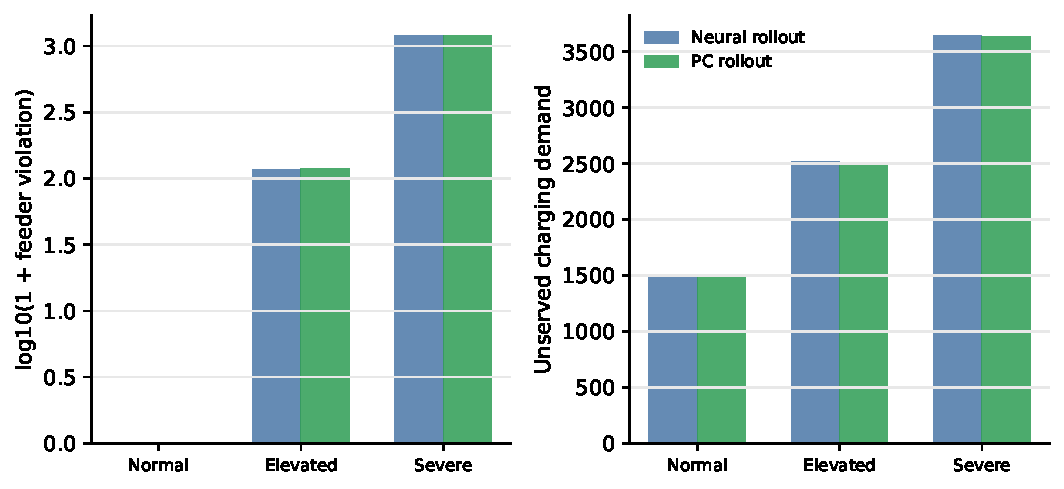
\includegraphics[width=0.98\linewidth]{fig_smartgrid_stress.pdf}
%DIFDELCMD < %%%
%DIFDELCMD < \caption{%
{%DIFAUXCMD
\DIFdelFL{Feeder margin violation and unserved charging demand under grid stress
cases.  The feeder margin panel uses $\log_{10}(1+\mathrm{value})$.}}
%DIFAUXCMD
%DIFDELCMD < \label{fig:smartgrid-stress}
%DIFDELCMD < \end{figure}
%DIFDELCMD < %%%
\DIFdelend \DIFaddbegin \DIFadd{Eleven independent checks connected the mathematical statements to the
numerical calculations.  Ten thousand
random score and budget tests preserved each continuous budget, with a maximum numerical
error of $1.37\times10^{-4}$.  Another 5,000 largest remainder tests preserved the
integer crew count.  All 8,117 nonzero 2023 test hours satisfied the analytical
zero service backlog bound.  A further 100,000 steps at simultaneous upper
uncertainty bounds remained inside $[0,0.98]^{3N}$.  All 14,902 standalone SMART-DS
projections, 147,456 primary online calls, and 36,864 stress online calls were
feasible after projection.  Packet backup and action derating checks had zero
logic error.  Every checked route visited each selected job once.  All main
crew counts matched completion event logs with paired inputs.  All 2,592
station choice flows met capacity.  The supporting map links each
property to its theorem, function, evidence file, and status.
}\DIFaddend 

\DIFdelbegin %DIFDELCMD < \input{table_restore_sensitivity}
%DIFDELCMD < 

%DIFDELCMD < %%%
\DIFdel{The grid stress cases extend the comparison beyond average cascade behavior.  In Table~\ref{tab:smartgrid-stress} and Fig.~\ref{fig:smartgrid-stress}, charging demand is increased and feeder margin is reduced, so feeder violation
and unserved charging both rise with stress level.  PC rollout remains below
neural rollout in cost across these cases,
although the relative gain becomes
smaller under the most severe feeder stress.  That change is important for
interpreting the result.  Restoration can reduce propagation through the communication and mobility layers, but it cannot create feeder capacity removed
by the stress setting.  The coupling cases give the complementary view.  Stronger
power to communication and communication to mobility coupling raises total cost,
while the PC rollout gain remains present because the envelope still shifts
restoration toward zones likely to transmit disturbance across domains.  }\DIFdelend \DIFaddbegin \subsection{\DIFadd{Interpretation and reproducibility}}
\DIFaddend 

\DIFdelbegin \DIFdel{Changing the restoration budget }\DIFdelend \DIFaddbegin

\DIFadd{The paired comparison identifies the value of transition evaluation rather
than the value of an additional demand forecast.  Central PC and the forecast
matched baseline receive the same forecast, current state, feeder mapping, work
orders, route candidates, and realized history.  Their difference is that
central PC propagates the calibrated transition before selecting a route.  The
overall improvement is modest, becomes larger in cascade and compound cases,
and remains in the same direction under the tested objective weights.  The
small nominal effect is consistent with the decision rule because future
propagation changes little when the initial threat is mild.
}

\DIFadd{The robust extension provides a separate comparison with central PC.  It has a
higher mean cost and does not reduce the reported conditional tail means or the
maximum cost.  The direct comparisons under altered transition coefficients
also favor central PC in the settings with resolved intervals.  These results
support the calibrated central transition as the principal model and retain the
finite worst set calculation as a sensitivity variant.  The distinction also
keeps the empirical conclusion aligned with the policy definitions }\DIFaddend in
Table~\DIFdelbegin \DIFdel{\ref{tab:restore-sensitivity} adds a second check on the same mechanism.  A larger budget lowers cost and improves
service continuity, while feeder violation changes only moderately because
local capacity and exogenous charging demand still constrain that term.
The
largest benefit comes from reducing communication loss and mobility delay during
cascading disturbances.  This ordering matches Theorem 1 and Corollary 1, which
identify propagation growth, stress feedback, and action sensitivity as the
quantities that control finite horizon risk.  PC rollout does not alter the demand forecast used by neural rollout.  It changes restoration so that future
cross domain exposure is smaller before the cascade becomes visible in the
current loss map.  }\DIFdelend \DIFaddbegin \DIFadd{\ref{tab:policy-definitions}.
}\DIFaddend 

\DIFaddbegin \DIFadd{Execution results explain the route from a requested decision to a realized
state.  At measured load, the feeder accepts every raw charging action.  Under
the electrical stress condition, projection reduces the request and transfers
curtailed energy to backlog.  The packet experiment shows that backup duration
changes the fraction of commands delivered on time and therefore changes
operating cost.  The crew experiment records repair only after an integer route
reaches the corresponding completion time.  Electrical feasibility is thus
calculated independently after policy scoring, while relative policy cost is
estimated from the stated service objective and transition scenarios.
}

\DIFadd{The three public data sources enter through distinct variables.  Boulder
transactions provide measured station arrivals and session energy.  EAGLE-I
provides county level event timing for transition calibration and service time
scenarios.  SMART-DS provides an independent feeder for charging feasibility.
Communication traffic and backup duration define controlled operating
conditions.  This arrangement forms a public data service restoration study
with a fixed feeder topology and explicit execution rules.
}

\DIFadd{The materials supporting these results are available in a public repository.
The repository provides the code, processed inputs, scenario level
outputs, trained model parameters, statistical results, distribution feeder,
route completion records, and packet records used in this study.  Source
metadata record the public origin, license, access date, byte count, and SHA256
value of each reused data collection.  Processed data retain variable
definitions, calendar splits, missing value rules, time zone conversion, and
energy conservation checks.  The repository also includes the software
environment, fixed initialization records, complete parameter table, and the
evidence needed to regenerate the principal statistics.  The repository is
available at
}\url{https://github.com/ahshicr/TSG-01697-2026-reproducibility}\DIFadd{.
}


\DIFaddend \section{Conclusion}

\DIFdelbegin \DIFdel{We studied rollout restoration for cyber physical smart grids coupled with
urban electric mobility.  PC rollout combines graph based charging state
forecasting, a physics guided digital twin, a monotone threat propagation }\DIFdelend \DIFaddbegin \DIFadd{This paper connects measured charging demand, a calibrated transition }\DIFaddend model,
and \DIFdelbegin \DIFdel{a concave restoration allocation rule.  The theoretical analysis gives a finite horizon risk bound that connects rollout performance to the propagation
growth factor.  The public city scale mobility experiment indicates that the method is most useful in cascading, compound, and stressed charging operation, while normal operation remains close to the neural rollout baseline.  Full year
training and repeated closed loop scenario evaluation benefit from parallel
graphics and central processor resources}\DIFdelend \DIFaddbegin \DIFadd{executable restoration decisions.  Central PC evaluates the future effect
of a candidate route while a matched baseline uses the same forecast and
current state without threat propagation}\DIFaddend .  \DIFaddbegin \DIFadd{The paired results show a consistent
cost reduction for central PC, with the clearest effect under cascade and
compound conditions.  The worst set extension does not improve the reported
mean or tail measures and is therefore retained as a sensitivity variant.
Packet delivery, distribution system projection, and integer crew completion
determine whether a main loop request changes the realized state.  A separate
capacity constrained assignment evaluates station reassignment.  The
mathematical results establish finite horizon sensitivity for the continuous
decision layer, a conditional bound for route selection, and feasibility
properties for executed actions.  The resulting closed loop model provides an
empirical and computational basis for studying service restoration across mobility,
distribution, communication, and repair operations.
}\DIFaddend 

\DIFaddbegin \IEEEtriggeratref{26}
\DIFaddend \bibliographystyle{IEEEtran}
\bibliography{references_latexdiff}

\end{document}
